\documentclass[11pt,fleqn,openany]{book}
\usepackage[utf8]{inputenc}
\usepackage[top=3cm,bottom=3cm,left=3.2cm,right=3.2cm,headsep=10pt,letterpaper]{geometry}
\usepackage{xcolor}
\definecolor{ocre}{RGB}{38,131,255}
\definecolor{ForestGreen}{RGB}{34,139,34}
\usepackage{avant}
\usepackage{mathptmx}
\usepackage{microtype}
\usepackage[T1]{fontenc}
\usepackage{inconsolata}
\usepackage{tabulary}

\usepackage[hidelinks]{hyperref} \def\UrlBreaks{\do\/\do-} % breaks long url in
% references
\usepackage{graphicx}
\usepackage[english]{babel}
\usepackage{listings}
\usepackage{listings-golang}
\usepackage{color}
\usepackage{tikz}
\usepackage[labelfont=it,textfont={it},singlelinecheck=on,justification=centering]{caption}
\usepackage{amsmath}
\usepackage{float}
\usepackage{comment}
\usepackage{cite}

\lstset{basicstyle=\ttfamily\footnotesize,breaklines=true}
\lstset{numbers=left,numberstyle=\tiny, stepnumber=1, numbersep=5pt}
\lstset{language=TeX}
\setlength{\parskip}{1em}

\renewcommand{\baselinestretch}{1.2}

\newcommand{\x}[1]{{\tt #1}} \newcommand{\code}[1]{{\em #1}}
\newcommand{\todo}[1]{{\color{red} TODO #1 }}
\newcommand{\bs}[1]{{\color{red}#1}}

\lstset{ % add your own preferences
    basicstyle=\footnotesize\tt,
    keywordstyle=\color{blue},
    numbers=left,
    numbersep=5pt,
    showstringspaces=false,
    stringstyle=\color{red},
    commentstyle=\color{ForestGreen},
    tabsize=2,
    language=Golang
}

\title{\textbf{\sffamily\color{white} \
Storj: A Decentralized Cloud Storage Network Framework}}
\author{\small\sffamily\color{white}
Storj Labs, Inc.}
\date{\small\sffamily\color{white} v3.0, September 17, 2018\\
\small\color{white}\url{https://github.com/storj/whitepaper}
}

%----------------------------------------------------------------------------------------
%	VARIOUS REQUIRED PACKAGES
%----------------------------------------------------------------------------------------

\usepackage{titlesec} % Allows customization of titles

\graphicspath{{Pictures/}} % Specifies the directory where pictures are stored

\usepackage{enumitem} % Customize lists
\setlist{nolistsep} % Reduce spacing between bullet points and numbered lists

\usepackage{booktabs} % Required for nicer horizontal rules in tables

\usepackage{eso-pic} % Required for specifying an image background in the title page

%----------------------------------------------------------------------------------------
%	MAIN TABLE OF CONTENTS
%----------------------------------------------------------------------------------------

\usepackage{titletoc} % Required for manipulating the table of contents

\contentsmargin{0cm} % Removes the default margin
% Chapter text styling
\titlecontents{chapter}[1.25cm] % Indentation
{\addvspace{15pt}\large\sffamily\bfseries} % Spacing and font options for chapters
{\color{ocre!60}\contentslabel[\Large\thecontentslabel]{1.25cm}\color{ocre}} % Chapter number
{}
{\color{ocre!60}\normalsize\sffamily\bfseries\;\titlerule*[.5pc]{.}\;\thecontentspage} % Page number
% Section text styling
\titlecontents{section}[1.25cm] % Indentation
{\addvspace{5pt}\sffamily\bfseries} % Spacing and font options for sections
{\contentslabel[\thecontentslabel]{1.25cm}} % Section number
{}
{\sffamily\hfill\color{black}\thecontentspage} % Page number
[]
% Subsection text styling
\titlecontents{subsection}[1.25cm] % Indentation
{\addvspace{1pt}\sffamily\small} % Spacing and font options for subsections
{\contentslabel[\thecontentslabel]{1.25cm}} % Subsection number
{}
{\sffamily\;\titlerule*[.5pc]{.}\;\thecontentspage} % Page number
[]

%----------------------------------------------------------------------------------------
%	MINI TABLE OF CONTENTS IN CHAPTER HEADS
%----------------------------------------------------------------------------------------

% Section text styling
\titlecontents{lsection}[0em] % Indendating
{\footnotesize\sffamily} % Font settings
{}
{}
{}

% Subsection text styling
\titlecontents{lsubsection}[.5em] % Indentation
{\normalfont\footnotesize\sffamily} % Font settings
{}
{}
{}

%----------------------------------------------------------------------------------------
%	PAGE HEADERS
%----------------------------------------------------------------------------------------

\usepackage{fancyhdr} % Required for header and footer configuration

\pagestyle{fancy}
\renewcommand{\chaptermark}[1]{\markboth{\sffamily\normalsize\bfseries\chaptername\ \thechapter.\ #1}{}} % Chapter text font settings
\renewcommand{\sectionmark}[1]{\markright{\sffamily\normalsize\thesection\hspace{5pt}#1}{}} % Section text font settings
\fancyhf{} \fancyhead[LE,RO]{\sffamily\normalsize\thepage} % Font setting for the page number in the header
\fancyhead[LO]{\rightmark} % Print the nearest section name on the left side of odd pages
\fancyhead[RE]{\leftmark} % Print the current chapter name on the right side of even pages
\renewcommand{\headrulewidth}{0.5pt} % Width of the rule under the header
\addtolength{\headheight}{2.5pt} % Increase the spacing around the header slightly
\renewcommand{\footrulewidth}{0pt} % Removes the rule in the footer
\fancypagestyle{plain}{\fancyhead{}\renewcommand{\headrulewidth}{0pt}} % Style for when a plain pagestyle is specified

% Removes the header from odd empty pages at the end of chapters
\makeatletter
\renewcommand{\cleardoublepage}{
\clearpage\ifodd\c@page\else
\hbox{}
\vspace*{\fill}
\thispagestyle{empty}
\newpage
\fi}

%----------------------------------------------------------------------------------------
%	THEOREM STYLES
%----------------------------------------------------------------------------------------

\usepackage{amsmath,amsfonts,amssymb,amsthm} % For math equations, theorems, symbols, etc

\newcommand{\intoo}[2]{\mathopen{]}#1\,;#2\mathclose{[}}
\newcommand{\ud}{\mathop{\mathrm{{}d}}\mathopen{}}
\newcommand{\intff}[2]{\mathopen{[}#1\,;#2\mathclose{]}}
\newtheorem{notation}{Notation}[chapter]

%%%%%%%%%%%%%%%%%%%%%%%%%%%%%%%%%%%%%%%%%%%%%%%%%%%%%%%%%%%%%%%%%%%%%%%%%%%
%%%%%%%%%%%%%%%%%%%% dedicated to boxed/framed environements %%%%%%%%%%%%%%
%%%%%%%%%%%%%%%%%%%%%%%%%%%%%%%%%%%%%%%%%%%%%%%%%%%%%%%%%%%%%%%%%%%%%%%%%%%
\newtheoremstyle{ocrenumbox}% % Theorem style name
{0pt}% Space above
{0pt}% Space below
{\normalfont}% % Body font
{}% Indent amount
{\small\bf\sffamily\color{ocre}}% % Theorem head font
{\;}% Punctuation after theorem head
{0.25em}% Space after theorem head
{\small\sffamily\color{ocre}\thmname{#1}\nobreakspace\thmnumber{\@ifnotempty{#1}{}\@upn{#2}}% Theorem text (e.g. Theorem 2.1)
\thmnote{\nobreakspace\the\thm@notefont\sffamily\bfseries\color{black}---\nobreakspace#3.}} % Optional theorem note
\renewcommand{\qedsymbol}{$\blacksquare$}% Optional qed square

\newtheoremstyle{blacknumex}% Theorem style name
{5pt}% Space above
{5pt}% Space below
{\normalfont}% Body font
{} % Indent amount
{\small\bf\sffamily}% Theorem head font
{\;}% Punctuation after theorem head
{0.25em}% Space after theorem head
{\small\sffamily{\tiny\ensuremath{\blacksquare}}\nobreakspace\thmname{#1}\nobreakspace\thmnumber{\@ifnotempty{#1}{}\@upn{#2}}% Theorem text (e.g. Theorem 2.1)
\thmnote{\nobreakspace\the\thm@notefont\sffamily\bfseries---\nobreakspace#3.}}% Optional theorem note

\newtheoremstyle{blacknumbox} % Theorem style name
{0pt}% Space above
{0pt}% Space below
{\normalfont}% Body font
{}% Indent amount
{\small\bf\sffamily}% Theorem head font
{\;}% Punctuation after theorem head
{0.25em}% Space after theorem head
{\small\sffamily\thmname{#1}\nobreakspace\thmnumber{\@ifnotempty{#1}{}\@upn{#2}}% Theorem text (e.g. Theorem 2.1)
\thmnote{\nobreakspace\the\thm@notefont\sffamily\bfseries---\nobreakspace#3.}}% Optional theorem note

%%%%%%%%%%%%%%%%%%%%%%%%%%%%%%%%%%%%%%%%%%%%%%%%%%%%%%%%%%%%%%%%%%%%%%%%%%%
%%%%%%%%%%%%% dedicated to non-boxed/non-framed environements %%%%%%%%%%%%%
%%%%%%%%%%%%%%%%%%%%%%%%%%%%%%%%%%%%%%%%%%%%%%%%%%%%%%%%%%%%%%%%%%%%%%%%%%%
\newtheoremstyle{ocrenum}% % Theorem style name
{5pt}% Space above
{5pt}% Space below
{\normalfont}% % Body font
{}% Indent amount
{\small\bf\sffamily\color{ocre}}% % Theorem head font
{\;}% Punctuation after theorem head
{0.25em}% Space after theorem head
{\small\sffamily\color{ocre}\thmname{#1}\nobreakspace\thmnumber{\@ifnotempty{#1}{}\@upn{#2}}% Theorem text (e.g. Theorem 2.1)
\thmnote{\nobreakspace\the\thm@notefont\sffamily\bfseries\color{black}---\nobreakspace#3.}} % Optional theorem note
\renewcommand{\qedsymbol}{$\blacksquare$}% Optional qed square
\makeatother

% Defines the theorem text style for each type of theorem to one of the three styles above
\newcounter{dummy}
\numberwithin{dummy}{section}
\theoremstyle{ocrenumbox}
\newtheorem{theoremeT}[dummy]{Theorem}
\newtheorem{problem}{Problem}[chapter]
\newtheorem{exerciseT}{Exercise}[chapter]
\theoremstyle{blacknumex}
\newtheorem{exampleT}{Example}[chapter]
\theoremstyle{blacknumbox}
\newtheorem{vocabulary}{Vocabulary}[chapter]
\newtheorem{definitionT}{Definition}[section]
\newtheorem{corollaryT}[dummy]{Corollary}
\theoremstyle{ocrenum}
\newtheorem{proposition}[dummy]{Proposition}

%----------------------------------------------------------------------------------------
%	DEFINITION OF COLORED BOXES
%----------------------------------------------------------------------------------------

\RequirePackage[framemethod=default]{mdframed} % Required for creating the theorem, definition, exercise and corollary boxes

% Theorem box
\newmdenv[skipabove=7pt,
skipbelow=7pt,
backgroundcolor=black!5,
linecolor=ocre,
innerleftmargin=5pt,
innerrightmargin=5pt,
innertopmargin=5pt,
leftmargin=0cm,
rightmargin=0cm,
innerbottommargin=5pt]{tBox}

% Exercise box
\newmdenv[skipabove=7pt,
skipbelow=7pt,
rightline=false,
leftline=true,
topline=false,
bottomline=false,
backgroundcolor=ocre!10,
linecolor=ocre,
innerleftmargin=5pt,
innerrightmargin=5pt,
innertopmargin=5pt,
innerbottommargin=5pt,
leftmargin=0cm,
rightmargin=0cm,
linewidth=4pt]{eBox}

% Definition box
\newmdenv[skipabove=7pt,
skipbelow=7pt,
rightline=false,
leftline=true,
topline=false,
bottomline=false,
linecolor=ocre,
innerleftmargin=5pt,
innerrightmargin=5pt,
innertopmargin=0pt,
leftmargin=0cm,
rightmargin=0cm,
linewidth=4pt,
innerbottommargin=0pt]{dBox}

% Corollary box
\newmdenv[skipabove=7pt,
skipbelow=7pt,
rightline=false,
leftline=true,
topline=false,
bottomline=false,
linecolor=gray,
backgroundcolor=black!5,
innerleftmargin=5pt,
innerrightmargin=5pt,
innertopmargin=5pt,
leftmargin=0cm,
rightmargin=0cm,
linewidth=4pt,
innerbottommargin=5pt]{cBox}

% Creates an environment for each type of theorem and assigns it a theorem text style from the "Theorem Styles" section above and a colored box from above
\newenvironment{theorem}{\begin{tBox}\begin{theoremeT}}{\end{theoremeT}\end{tBox}}
\newenvironment{exercise}{\begin{eBox}\begin{exerciseT}}{\hfill{\color{ocre}\tiny\ensuremath{\blacksquare}}\end{exerciseT}\end{eBox}}
\newenvironment{definition}{\begin{dBox}\begin{definitionT}}{\end{definitionT}\end{dBox}}
\newenvironment{example}{\begin{exampleT}}{\hfill{\tiny\ensuremath{\blacksquare}}\end{exampleT}}
\newenvironment{corollary}{\begin{cBox}\begin{corollaryT}}{\end{corollaryT}\end{cBox}}

%----------------------------------------------------------------------------------------
%	REMARK ENVIRONMENT
%----------------------------------------------------------------------------------------

\newenvironment{remark}{\par\vspace{10pt}\small % Vertical white space above the remark and smaller font size
\begin{list}{}{
\leftmargin=35pt % Indentation on the left
\rightmargin=25pt}\item\ignorespaces % Indentation on the right
\makebox[-2.5pt]{\begin{tikzpicture}[overlay]
\node[draw=ocre!60,line width=1pt,circle,fill=ocre!25,font=\sffamily\bfseries,inner sep=2pt,outer sep=0pt] at (-15pt,0pt){\textcolor{ocre}{R}};\end{tikzpicture}} % Orange R in a circle
\advance\baselineskip -1pt}{\end{list}\vskip5pt} % Tighter line spacing and white space after remark

%----------------------------------------------------------------------------------------
%	SECTION NUMBERING IN THE MARGIN
%----------------------------------------------------------------------------------------

\makeatletter
\renewcommand{\@seccntformat}[1]{\llap{\textcolor{ocre}{\csname the#1\endcsname}\hspace{1em}}}
\renewcommand{\section}{\@startsection{section}{1}{\z@}
{-4ex \@plus -1ex \@minus -.4ex}
{1ex \@plus.2ex }
{\normalfont\large\sffamily\bfseries}}
\renewcommand{\subsection}{\@startsection {subsection}{2}{\z@}
{-3ex \@plus -0.1ex \@minus -.4ex}
{0.5ex \@plus.2ex }
{\normalfont\sffamily\bfseries}}
\renewcommand{\subsubsection}{\@startsection {subsubsection}{3}{\z@}
{-2ex \@plus -0.1ex \@minus -.2ex}
{.2ex \@plus.2ex }
{\normalfont\small\sffamily\bfseries}}
\renewcommand\paragraph{\@startsection{paragraph}{4}{\z@}
{-2ex \@plus-.2ex \@minus .2ex}
{.1ex}
{\normalfont\small\sffamily\bfseries}}

%----------------------------------------------------------------------------------------
%	HYPERLINKS IN THE DOCUMENTS
%----------------------------------------------------------------------------------------

% For an unclear reason, the package should be loaded now and not later
\usepackage{hyperref}
\hypersetup{hidelinks,backref=true,pagebackref=true,hyperindex=true,colorlinks=false,breaklinks=true,urlcolor= ocre,bookmarks=true,bookmarksopen=false,pdftitle={Title},pdfauthor={Author}}

%----------------------------------------------------------------------------------------
%	CHAPTER HEADINGS
%----------------------------------------------------------------------------------------

% The set-up below should be (sadly) manually adapted to the overall margin page septup controlled by the geometry package loaded in the main.tex document. It is possible to implement below the dimensions used in the goemetry package (top,bottom,left,right)... TO BE DONE

\newcommand{\thechapterimage}{}
\newcommand{\chapterimage}[1]{\renewcommand{\thechapterimage}{#1}}

% Numbered chapters with mini tableofcontents
\def\thechapter{\arabic{chapter}}
\def\@makechapterhead#1{
\thispagestyle{empty}
{\centering \normalfont\sffamily
\ifnum \c@secnumdepth >\m@ne
\if@mainmatter
\startcontents
\begin{tikzpicture}[remember picture,overlay]
\node at (current page.north west)
{\begin{tikzpicture}[remember picture,overlay]
\node[anchor=north west,inner sep=0pt] at (0,0) {\includegraphics[width=\paperwidth]{\thechapterimage}};
%%%%%%%%%%%%%%%%%%%%%%%%%%%%%%%%%%%%%%%%%%%%%%%%%%%%%%%%%%%%%%%%%%%%%%%%%%%%%%%%%%%%%
% Commenting the 3 lines below removes the small contents box in the chapter heading
%\fill[color=ocre!10!white,opacity=.6] (1cm,0) rectangle (8cm,-7cm);
%\node[anchor=north west] at (1.1cm,.35cm) {\parbox[t][8cm][t]{6.5cm}{\huge\bfseries\flushleft \printcontents{l}{1}{\setcounter{tocdepth}{2}}}};
\draw[anchor=west] (5cm,-9cm) node [rounded corners=20pt,fill=ocre!10!white,text opacity=1,draw=ocre,draw opacity=1,line width=1.5pt,fill opacity=.6,inner sep=12pt]{\huge\sffamily\bfseries\textcolor{black}{\thechapter. #1\strut\makebox[22cm]{}}};
%%%%%%%%%%%%%%%%%%%%%%%%%%%%%%%%%%%%%%%%%%%%%%%%%%%%%%%%%%%%%%%%%%%%%%%%%%%%%%%%%%%%%
\end{tikzpicture}};
\end{tikzpicture}}
\par\vspace*{230\p@}
\fi
\fi}

% Unnumbered chapters without mini tableofcontents (could be added though)
\def\@makeschapterhead#1{
\thispagestyle{empty}
{\centering \normalfont\sffamily
\ifnum \c@secnumdepth >\m@ne
\if@mainmatter
\begin{tikzpicture}[remember picture,overlay]
\node at (current page.north west)
{\begin{tikzpicture}[remember picture,overlay]
\node[anchor=north west,inner sep=0pt] at (0,0) {\includegraphics[width=\paperwidth]{\thechapterimage}};
\draw[anchor=west] (5cm,-9cm) node [rounded corners=20pt,fill=ocre!10!white,fill opacity=.6,inner sep=12pt,text opacity=1,draw=ocre,draw opacity=1,line width=1.5pt]{\huge\sffamily\bfseries\textcolor{black}{#1\strut\makebox[22cm]{}}};
\end{tikzpicture}};
\end{tikzpicture}}
\par\vspace*{230\p@}
\fi
\fi
}
\makeatother


\begin{document}

\thispagestyle{fancy}
\chapterimage{images/header.eps}
\AddToShipoutPicture*{\put(0,0){
\includegraphics[width=\paperwidth]{images/front.eps}}}

\maketitle

\begin{tikzpicture}[remember picture,overlay]
\node[rotate=45,scale=15,text opacity=0.1]
at (current page.center) {DRAFT};
\end{tikzpicture}

\newpage

\tableofcontents\newpage

\section{Abstract}

Decentralized cloud storage represents a fundamental shift in
the efficiency and economics of large-scale storage.
Eliminating central control allows users to store and share data
without reliance on a third-party storage provider. Decentralization mitigates
the risk of data failures and outages while simultaneously increasing
the security and privacy of object storage, while also
allowing market forces to optimize on cheaper ways to
provide storage at a greater rate than any single entity could afford.
Though there are many ways to build such a system, there are some specific
responsibilities any given implementation should address.
Based on our experience with petabyte-scale
storage systems, we introduce a modular framework for considering these
responsibilities and building our distributed storage network.
Additionally, we describe an initial
concrete implementation for the entire framework.

\section{Contributors}

This paper represents the combined efforts of many individuals.
Contributors at Storj Labs, Inc. include but are not limited to:
Alexander Bender,
Alexander Leitner,
Ben Golub,
Benjamin Sirb,
Brandon Iglesias,
Bryan White,
Cameron Ayer,
Dan Sorensen,
Dennis Coyle,
Dylan Lott,
Egon Elbre,
Garrett Ransom,
Helene Unland,
James Hagans,
Jennifer Johnson,
Jens Heimbürge,
John Gleeson,
Jon Sanderson,
JT Olio,
Kaloyan Raev,
Kevin Leffew,
Kishore Aligeti,
Matthew Robinson,
Maximillian von Briesen,
Nadine Farah,
Natalie Villasana,
Patrick Gerbes,
Paul Cannon,
Philip Hutchins,
Shawn Wilkinson,
Stefan Benten,
Tim Adams,
and Viktor Ihnatiuk.

We'd also like to especially thank the other authors of the previous
Storj v2 whitepaper:
Braydon Fuller,
Chris Pollard,
Gordon Hall,
James Prestwich,
Josh Brandoff,
and Tome Boshevski.

Finally, we extend a huge thank you to everyone we talked to during the
design and architecture of this system for their valuable thoughts, feedback,
input, and suggestions.

\chapter{Introduction}

\todo{
Outline of this intro (and the entire paper) should be:
\begin{itemize}
\item Decentralized storage solves some big problems.
\item Decentralized storage addresses a specific market we're interested in.
\item To best address this market, our product must satisfy specific constraints.
\item We believe a specific framework is required to best satisfy these
  constraints. We will not need a v4 as this framework is fairly fundamental
  to our space.
\item Our concrete implementation is just one potential solution within our
  framework. We plan to improve our implementation within the framework over
  time.
\item We have made a product out of these concrete framework choices.
\end{itemize}
}

The Internet is a massive decentralized and distributed network consisting of
billions of devices which are not controlled by a single group or entity.
However, much of the data available through the Internet is quite centralized,
currently stored with a handful of technology companies that have the
experience and capital to build massive data centers capable of handling this
vast amount of information.
In recent years, we have seen colossal infrastructure data breaches, periods of
unavailability on a grand scale, storage costs failing to decrease in line with
demand, and a struggle to keep up with user demand for faster data and larger
formats.

\todo{Cam suggests for the next paragraph:
I think it would be better to start with the problem, "there is expected to be X amount of data by year Y." Then propose decentralized storage as a potential solution. Start general, then progressively get more specific until you reach the thesis, "Storj is the answer"
}

Decentralized storage has emerged as an answer to the challenge of
providing a performant, secure, private, and economical cloud storage solution.
Decentralized storage can do this because its architecture matches the real
Internet better, which itself is decentralized, as opposed to massive
centralized data centers. This model can address the rapidly
expanding amount of data for which current solutions struggle.
With an anticipated 44 zettabytes of data expected to exist by 2020 and a
market that will grow to \$92 billion USD in the same time frame
\todo{citations needed}, we have discovered that decentralized cloud storage
has the potential to address several key market segments.
As the industry's capabilities evolve, decentralized cloud
storage will be able to address a much wider range of use cases from basic
object storage to content delivery networks (CDN).

Decentralized cloud storage is rapidly advancing in maturity, but its evolution
is subject to a specific set of design constraints which
define the overall requirements and implementation of
the network. When designing a distributed storage system,
there are many parameters to be optimized such as speed, capacity,
trustlessness, byzantine fault tolerance, cost, bandwidth, and latency.

We propose a framework that scales horizontally to serve hundreds of millions of
people across the globe. Our system, the Storj Network, is a robust object store
that encrypts, shards, and distributes data to nodes across the globe for
storage.
Data is served in a manner purposefully designed to prevent
breaches.
In order to accomplish this task, we've designed our system to be modular,
consisting of independent components with task-specific jobs.
We've integrated these components to implement a decentralized object storage
system that is secure, performant, and reliable.

We have organized the rest of this paper into six
chapters: chapter \ref{chap:design-constraints} discusses the design space
in which Storj operates and elaborates on specific constraints which
we base our optimization efforts on.
Chapter \ref{chap:framework} covers our framework, while chapter
\ref{chap:concrete}
proposes a simple concrete implementation of each component.
Chapter \ref{chap:walkthroughs} explains what happens
during each operation in the network. Finally, chapter
\ref{chap:future-work} covers future areas of research.

\chapter{Storj design constraints}\label{chap:design-constraints}

Before designing a system, it's important to first define its requirements.
There are many different ways to design a decentralized storage system, but
with the addition of a few requirements, the potential design space shrinks
significantly.
Our design constraints are heavily influenced by our product and
market fit goals.
By carefully considering each requirement, we ensure the framework
we choose is as universal as possible, given the constraints.

\section{S3 compatibility}

At the time of publishing this paper, the most widely deployed cloud storage
protocol is Amazon Web Services' Simple Storage Service protocol, or S3 for
short. Most cloud storage products provide some form of compatibility with the
S3 API architecture.

Our objective is to aggressively compete in the wider cloud
storage industry and bring decentralized cloud storage into the mainstream.
Until a decentralized cloud storage protocol becomes widely adopted,
we are creating a graceful transition path from centralized
providers for our users.
This will alleviate many switching costs for users with data currently stored on
a centralized provider.
To achieve this, the Storj implementation allows
applications previously built against S3 to work with Storj with
minimal friction or changes.
This adds strong requirements on feature set, performance, and durability.
At a bare minimum, this requires the methods sketched out in
Figure \ref{fig:s3-api-code} to be implemented.

\begin{figure}
\begin{lstlisting}
  // Bucket operations
	CreateBucket(bucketName string)
	DeleteBucket(bucketName string)
	ListBuckets() []BucketInfo

  // Object operations
	GetObject(bucketName, objectPath string, offset, length int64) (
	    ObjectData, ObjectInfo)
	PutObject(bucketName, objectPath string, data ObjectData,
	    metadata map[string]string) ObjectInfo
	DeleteObject(bucketName, objectPath string)
	ListObjects(bucketName, prefix, startKey string,
	    limit int, recursive bool) ([]ObjectInfo, more bool)
\end{lstlisting}
\caption{Minimum S3 API}
\label{fig:s3-api-code}
\end{figure}

\section{Device failure and churn}

For all devices, component failure is a guarantee.
All hard drives fail after enough wear
\cite{backblaze-hd-2018-q1} and servers providing network access to
these hard drives will eventually fail, too. Network links may die, power
failures could cause havoc sporadically,
and storage media become unreliable over time.
Data must be stored with enough redundancy to recover from
individual component failures.
Perhaps more importantly, no data can be left in a single location
indefinitely. In such an environment, redundancy, data
maintenance, repair, and replacement of lost redundancy must be considered
facts of life, and the system must account for these issues.

Furthermore, decentralized systems are susceptible to high churn rates, where
participants join the network and then leave for various reasons, well
before their hardware has actually failed. A network with a high churn rate will
use large amounts of bandwidth just to ensure durability of the data and
will fail to scale. As a result, a scalable, highly durable storage
network must encourage stable nodes and keep the churn rate as low as possible.

Churn rate affects the network much more than hardware failure. As an
illustration, Maymounkov {\em et al.} found that in
decentralized systems, the probability of a node staying connected to the
network for an additional hour is an {\em increasing}
function of uptime (Figure \ref{fig:kad-uptime} \cite{kad}).
In other words, the longer a node is a
participant in the network, the more likely it is to continue
participating. This gives our system a strong incentive to prefer long-lived
and stable nodes.

\begin{figure}
\centering
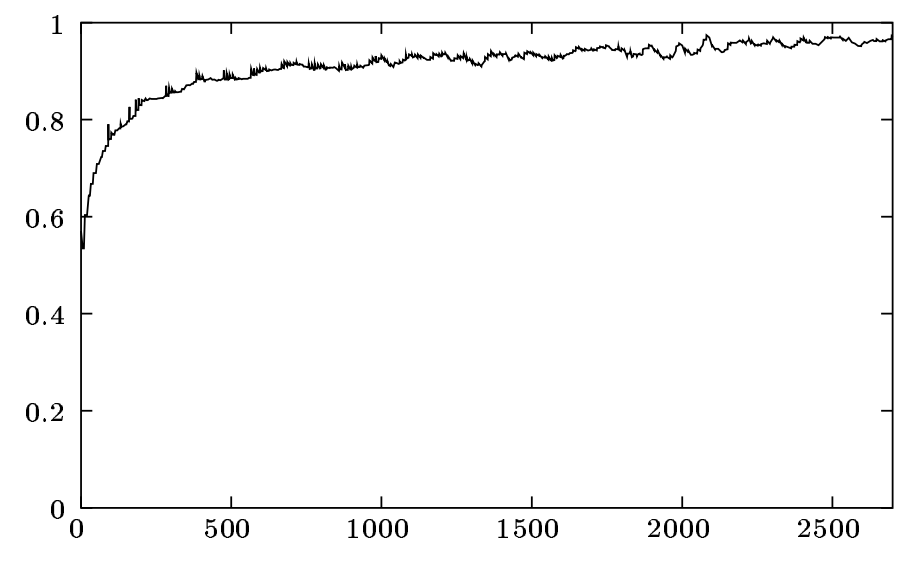
\includegraphics[width=.6\textwidth]{images/uptime.png}
\caption{Probability of remaining online an additional hour as a function of
uptime.
The $x$ axis represents minutes. The $y$ axis shows the fraction of nodes
that stayed online at least $x$ minutes that also stayed online at least
$x+60$ minutes. Source: Maymounkov {\em et al.} \cite{kad}}
\label{fig:kad-uptime}
\end{figure}

See Appendix \ref{appendix:RS} for a discussion about how repair bandwidth
varies as a function of node churn.

\section{Latency}

Unlike traditional data centers,
decentralized storage systems can potentially capitalize on
massive opportunities for parallelism.
Some of these opportunities include increased transfer rates, processing
capabilities, and overall throughput even when individual
network links are slow. However, parallelism cannot, by itself, improve {\em
latency}. If an individual network link is utilized as part of an operation,
its latency will be the lower bound for the overall operation.
Therefore, any distributed system
intended for high performance applications must continuously and aggressively
optimize for low latency, both at an individual process scale, as well as for
the system's entire architecture.

\section{Bandwidth}\label{sec:req-bandwidth}

Global bandwidth availability is increasing year after year; but unfortunately,
access to
high-bandwidth internet connections is unevenly distributed across the world.
While some users can easily access symmetric, high-speed, unlimited bandwidth
connections, others may have significant difficulty obtaining access to the same.

In the United States and other countries,
the way many residential internet service providers (ISPs)
operate presents two specific challenges for designers of a
decentralized network protocol. The first challenge designers often face are
the asymmetric internet connections offered by ISPs.
Customers subscribe to internet service
based on an advertised download speed, but the upload speed is potentially an
order of magnitude or two slower. The second challenge is that bandwidth is
sometimes "capped" by the ISP at a fixed amount of allowed traffic per month.
For example, in many
US markets, the ISP Comcast imposes a one terabyte per month bandwidth cap
with stiff fines for customers who go over this limit \cite{comcast-cap}.
An internet connection with a cap of 1 TB/month cannot average more than
385 KB/s over the month without exceeding the monthly bandwidth allowance,
even if the ISP advertises speeds of 10 MB/s or higher.
Such caps impose
significant limitations on the bandwidth available to the network
at any given moment.

With device failure and churn guaranteed, any decentralized system will have a
corresponding amount of repair traffic. As a result, it is important to account
for the bandwidth required not only for data storage and retrieval, but also
for data maintenance and repair. Designing a
storage system that is careless with bandwidth usage would give undue
preference to storage node operators with access to unlimited high-speed
bandwidth, centralizing the system to some degree. In order to keep the storage
system as decentralized as possible and working in as many environments
as possible, bandwidth usage must be aggressively minimized.

Please see appendix \ref{appendix:bandwidth-space-limits} for a discussion on how
bandwidth availability and repair traffic limit usable space.

\section{Security and privacy}

One of the primary focuses of the Storj network is to ensure that its users'
data privacy is protected. This is not addressed as an afterthought but is
built into the design of the clients, network, and other related services.

Any object storage platform in our market should ensure both the privacy and
security of data stored; however,
decentralized storage platforms include an additional layer of
complexity and risk associated with the storage of data on inherently
untrusted nodes. Because decentralized storage platforms cannot take many
of the same shortcuts data center based approaches can (e.g. firewalls, DMZs,
etc.), decentralized storage must be designed from the ground up to support
enhanced security and privacy at all levels of the system.

Data security encompasses a wide range of concerns including
identity and access management, prevention of tampering or unauthorized
modification, prevention of ransomware attacks, system vulnerabilities, and
malicious insiders. Data privacy, on the other hand, includes storage of data
without providing access to the underlying data and its metadata by
Storj Labs, third-party operators of system components, or malicious actors.

Certain categories of data are subject to specific regulatory compliance.
For example, legislation in the United States includes
the Health Insurance Portability and
Accountability Act (HIPAA) which has requirements for data center
compatibility. European countries have to consider the General Data Protection
Regulation (GDPR) regarding
how individual information must be protected and secured. Of course there
are many other regulations in other sectors.

Open source software
provides the level of transparency and assurance needed to prove that the
behaviors of the system are as advertised. Customers should be able to
evaluate that our software is implemented correctly, is resistant to
attack vectors (known or unknown), is secure, and otherwise fulfills all
of the customers' requirements.

\section{Object size}

We can broadly classify large storage systems into two groups by average
object size. When storing many small pieces of information, a
database is generally the preferred solution.
On the other hand, when storing many large
files, an object store or filesystem is ideal. We classify a "large" file as a
few megabytes or greater in size.

The initial product offering by Storj Labs is designed to function primarily as
a decentralized object store for larger files.
While future improvements may enable
database-like use cases, object storage is the predominant use case described in
this paper. We made protocol design decisions with the assumption that the
vast majority of stored objects will be four megabytes or larger.

It is worth pointing out that this will not negatively impact use cases that
require reading lots of files smaller than a megabyte. Users can address this
with a packing strategy, by aggregating and storing many small files as one
large file.
As the protocol supports seeking and streaming, users can download small files
without requiring full retrieval of the aggregated object.

\section{Decentralization}

Informally, a decentralized application is a service that has no single
operator. Furthermore, no single entity should be solely responsible for the
cost associated with running the service.

One of the main motivations for preferring decentralization is to drive
down infrastructure costs for maintenance, utilities, and bandwidth.
We believe that there
are significant underutilized resources at the edge of the network and at
the margin for many smaller operators. In our experience building decentralized
storage networks, we have found a long tail of resources that are presently
unused or underused that could provide affordable and
geographically distributed cloud storage. Perhaps some small operator
has access to cheaper electricity than standard data centers or another small
operator has access to cheaper cooling. Many of these small operator
environments are not substantial enough to run an entire datacenter-like
storage system. However, we have found that in aggregate, enough small operator
environments exist such that their combination over the internet constitutes
significant opportunity and advantage for cheaper and faster storage.

Operating a decentralized network requires node operators to contribute
resources (e.g. network bandwidth, compute, storage, and energy) in exchange
for compensation (i.e. the opportunity to earn revenue).
In most instances, an increase in demand for a decentralized service drives
increase in adoption and proliferation of storage nodes.
This effectively increases the available capacity while at the same time
driving costs down.

Our decentralization goals are also driven by our desire to detangle
fundamental infrastructure (such as storage) from the hands of a few major
entities.
We believe that there exists inherent risk in trusting a single entity,
company, or organization with a significant fraction of the world's data.
In fact, we believe that there is an implicit cost associated with the risk of
trusting any third party with custodianship of personal data.

To illustrate, we find that there exists an array of unfavorable
and costly outcomes which may result from trusting a single entity.
For example, changes to the company's roadmap may result in the product
becoming less useful, changes to the company's position on data collection could
cause it to sell customer metadata to advertisers, or perhaps the company goes
out of business or otherwise fails to keep customer data safe.
By creating an equivalent or better decentralized
system, many users worried about single-entity risk will have a viable
alternative.
With decentralized architecture, Storj could cease operating and the data
would continue to be available.

We have decided to adopt a decentralized architecture because while there
are tradeoffs, we believe decentralization addresses the core limitations,
risks, and cost factors that result from centralized cloud storage.
Within this context,
decentralization results in a globally distributed singleton network that can
serve a wide range of storage use case from archival to CDN, whereas
centralized storage systems require different architectures, implementations
and infrastructure to address each of those same use cases.

\section{Byzantine fault tolerance}

Unlike centralized solutions like Amazon S3, Storj operates in an untrusted
environment, where individual storage providers are not necessarily assumed to be
trustworthy. Storj operates over the public internet, allowing anyone to sign
up to become a storage provider.

We adopt the BAR (Byzantine, Altruistic, Rational) model \cite{bar} to discuss
participants in the network.
{\em Byzantine} nodes may deviate arbitrarily from the suggested protocol for
any reason. Some examples include nodes that are broken or nodes that
are actively trying to sabotage the protocol. In general, a Byzantine node is
one that optimizes for a utility function that is independent of the one
given for the suggested protocol.
Inevitable hardware failures aside, {\em Altruistic} nodes
participate in a proposed protocol even if the rational choice is to deviate.
{\em Rational} nodes participate or deviate only when it
is in their net best interest to do so.

Some distributed storage systems (e.g. AWS S3, Azure Blob Storage)
operate in an environment
where all nodes are considered altruistic. For example, sans hardware failure
or security breaches, Amazon's storage nodes
are not going to do anything besides what they were explicitly programmed to do,
because Amazon owns and runs all of them.

On the other hand, Storj operates in an environment where every node is
managed by its own independent operator.
In this environment we can expect that a majority
of storage nodes are rational and a minority are byzantine. Storj assumes no
altruistic nodes.

\section{Coordination avoidance}\label{sec:coordination-avoidance}

A growing body of distributed database research shows that systems that
avoid coordination wherever possible have far better throughput than systems
where subcomponents are forced to coordinate to achieve correctness
\cite{cap1, cap2, consistency-vs-latency, hat, i-confluence, anna,
calm1, calm2}.
We continue using Bailis {\em et al.}'s informal definition
that coordination is the requirement that concurrently executing operations
synchronously communicate or otherwise stall in order to complete
\cite{i-confluence}.
This observation happens at all scales and applies not only to distributed
networks but also to
concurrent threads of execution coordinating within the same computer.
As soon as coordination is needed, actors in the system will need to wait for
other actors, and waiting due to coordination issues can be significantly
costly.

While many types of operations in a network may require coordination
(e.g., operations that require linearizability\footnote{
Linearizable operations are atomic operations on a specific object where
the order of operations is equivalent to the order given original "wall clock"
time.
}
\cite{jepsen-consistency, hat, vv-consistency}), choosing strategies that
avoid coordination (such as Highly Available Transactions \cite{hat}) can offer
performance gains of two to three orders of magnitude over wide area networks.
In fact, by carefully avoiding coordination as much as possible, the Anna
database is able to be 10 times faster than both Cassandra and Redis in their
corresponding environments, and 700 to 800 times faster than
performance-focused in-memory databases such as Masstree or TBB
\cite{anna, anna-announce}.
Not all coordination can be avoided, but new frameworks such as Invariant
Confluence \cite{i-confluence} allow system architects to understand when
coordination is required for consistency and correctness. As evidenced
by Anna's performance successes, it is most efficient to avoid coordination
where possible.

Systems that minimize coordination are
much better at scaling from small
to large workloads. Adding more resources to a coordination-avoidant system
will directly increase throughput and performance. On the other hand,
adding more resources to a coordination-dependent system
(such as Bitcoin \cite{bitcoin} or even Raft \cite{raft}) will not result in
additional throughput or overall performance.

To get to exabyte scale, minimizing coordination is one of the key components
of our strategy.
Surprisingly, many decentralized storage platforms are working towards
architectures that require significant amounts of coordination,
where most if not all operations must be accounted for by a single global
ledger. For us to achieve exabyte scale, it is a fundamental
requirement to limit hotpath coordination domains to small spheres,
entirely controllable by each user.

\section{Marketplace and economics}

Public cloud computing in general (and public cloud storage in particular) has
proven to be an attractive business model for the large centralized cloud
providers. Cloud computing is estimated to be a \$186.4 billion dollar market
in 2018, reaching \$302.5 billion by 2021 \cite{gartner-cloud-growth}.

The public cloud storage model has provided a compelling economic model to end
users by enabling them to scale on demand and avoid the significant fixed
costs associated with investments in facilities, power, and data center
personnel. Public cloud storage has generally proven to be an economical,
durable, and performant option for many end users, when compared to
on-premise solutions.

However, the public cloud storage model has, by its nature, led to a high
degree of concentration. Fixed costs are born by the network operators, who
invest billions of dollars in building out a network of data centers, and who
then enjoy significant economies of scale. The combination of large upfront
costs and economies of scale means that there is an extremely limited number
of viable suppliers of public cloud storage (arguably, less than 5 major
options worldwide). These few supplies are also the primary beneficiaries of
the economic return.

We believe that decentralized storage can provide a viable alternative to
centralized cloud.

In our design of Storj, we seek to create an economically advantageous
situation for four different groups:

\begin{description}
\item[End users] - We must provide the same economically compelling
  characteristics of public cloud. (No upfront costs, scale on demand).
  In addition, end users must experience meaningfully better value for given
  levels of capacity, durability, security, and performance.

\item[Storage node operators] - It must be economically attractive for storage
  node operators to help build out the network.
  They must be paid fairly and transparently, and be able to make a
  reasonable profit relative to any marginal costs they incur.
  At a bare minimum, it should be economically advantageous to be a storage
  node operator to utilize underused capacity, but we believe it should be
  economically advantageous to create new capacity as well.
  As node availability and reliability has a large impact on network
  availability, cost, and reliabilty, it is a requirement that storage node
  operators have sufficient incentive to maintain reliable and continuous
  connections to the network.

\item[Demand providers] - It must be economically attractive for developers and
  businesses to drive customers and data onto the Storj network. We will design
  the system to fairly and transparent deliver margin to partners. We believe
  that there is a unique opportunity to provide open-source software (OSS)
  companies and projects (who drive over $2/3$ of the public cloud workloads
  today without receiving direct revenue) a source of sustainable revenue.

\item[Network operator] - In order to sustain continued investment in code,
  functionality, network maintainance, and demand generation, the network
  operator must be able to retain a reasonable profit while charging end
  users less than the public cloud providers and sharing margin with storage
  node operators and demand providers.
\end{description}

Targeting these four groups constrains our design in a few ways.

First, it is important to distinguish supply and demand in regards to the
storage network; sharing resources with the network should be considered
separately from storing data on the network. This is because
the overwhelming majority of potential partners and customers who will
pay to store data on the
network do not also have a corresponding supply of storage space to share.

Second, individuals providing the supply of unused storage must
be compensated fairly in an easily calculable way.
This includes aligning the economic incentives of the network to ensure
that the {\em rational} nodes on the network (the majority of operators) behave
as similarly as possible to the expected behavior of {\em altruistic} nodes.
Incentives that allow for or encourage {\em byzantine} behavior should likewise
be eliminated.

Third, to drive network growth and adoption, we must have a price-competitive
product and attractive
opportunities available for demand-side partners. To create additional
incentives for partners or customers to bring data to the network,
the price charged for storage and bandwidth--combined with the other
benefits of decentralized storage--must be
more compelling and economically beneficial than competing storage solutions.

The network must be able to account for ensuring efficient and timely billing
and payment processes and regulatory compliance for tax and other reporting.
Decentralized application architectures have seen growing adoption of
cryptocurrencies for use in the transmission of value in
exchange for utilization of shared resources on the network.
In this case, Storj has implemented the STORJ token.
This presents the additional requirement that the network be able to process
an extremely large volume of cryptocurrency transactions.

Building a network of contributors will increase the ability to bring new
capabilities to market faster.
Because Storj is open source, the network must account for the operation of
servers by unaffiliated third parties and must be able to coordinate payment
as well as aggregate reputation data between numerous external network
components.

Due to the global network of supply and demand for storage and bandwidth, the
network must be able to transact in virtually any form of value whether that it
be fiat currency, cryptocurrency or some other form of barter.

Finally, the Storj roadmap will be aligned with the economic drivers of the
network.
New features and changes to the concrete implementations of framework
components will be driven by applicability to specific object storage use cases
and the relationship between features and performance to the price of storage
and bandwidth relative to those use cases.

\chapter{Framework}\label{chap:framework}

After having considered our design constraints, the next goal is to design
a framework consisting of relatively fundamental components.
The framework should describe
all of the components that must exist to satisfy our constraints.
As long as our design constraints remain constant, this framework will, as
much as is feasible, describe Storj now and Storj in 10 years from now.
While there will be significant design freedom within the framework,
this framework will obviate the need for future rearchitectures entirely, as
independent components will be able to replaced without affecting other
components.

\section{Framework overview}

All designs within our framework will do the following things:

\begin{description}

\item[Store data] When data is stored with the network, a client encrypts
and breaks it up into multiple pieces. The pieces are distributed
to peers across the network. When this happens, metadata is generated that
contains information on where to find the data again.

\item[Retrieve data] When data is retrieved from the network,
the client will first reference the metadata to identify the locations of the
previously stored pieces.
Then the pieces will be retrieved and the original data will be reassembled
on the client's local machine.

\item[Maintain data] When the amount of redundancy drops below a certain
threshold, the necessary data for the missing pieces is regenerated and
replaced.

\item[Pay for usage] A unit of value should be sent in exchange for
services rendered.

\end{description}

To improve understandability, we break up the design into a collection of
relatively independent concerns and then combine them to form the desired
framework.

The individual components are:

\begin{enumerate}
\item Storage nodes
\item Peer-to-peer communication and discovery
\item Redundancy
\item Metadata
\item Encryption
\item Audits and reputation
\item Data repair
\item Payments
\end{enumerate}

\section{Storage nodes}

The storage node's role is to store and return data.
Aside from reliably storing data, nodes should provide
network bandwidth and appropriate responsiveness.
Storage nodes are selected to store data based on various criteria: ping time,
latency, throughput, bandwidth caps, sufficient disk space,
geographic location, uptime, history of responding accurately to audits, etc.
In return for their service, nodes are rewarded for their participation via
payments.

Because storage
nodes are selected via changing variables external to the protocol, node
selection is an explicit, nondeterministic process in our framework. This means
that we must keep track of which nodes were selected for each upload via a
small amount of metadata; we can't select nodes for storing data implicitly or
deterministically as in a system like Dynamo \cite{dynamo}. This decision
implies the requirement of a metadata storage system to keep track
of selected nodes.

\section{Peer-to-peer communication and discovery}

All peers on the network communicate via a standarized protocol. The
framework requires that this protocol:

\begin{itemize}
\item provides peer reachability, even in the face of firewalls
and NATs where possible.
This may require techniques like STUN, UPnP, NAT-PMP, etc.
\item provides authentication, where each participant cryptographically
proves the identity of the peer with whom they are speaking to avoid
man-in-the-middle attacks.
\item provides complete privacy. In cases such as the bandwidth allocation
protocol (see section \ref{bap}), the client and storage node must be able
to communicate without any risk of eavesdroppers. The protocol should
ensure that all communications are private by default.
\end{itemize}

Additionally, the framework requires a way to look up peer network addresses
by a unique identifier so that, given a peer's network address, any other
peer can connect to it. This responsibility is similar to the internet's
standard domain name system (DNS), which is a mapping of an identifier to an
ephemeral connection address, but unlike DNS, there is no centralized
registration process.
To achieve this, a network overlay can be
built on top of our peer-to-peer communication protocol that provides this
functionality. See Section \ref{sec:concrete-node-discovery} for
implementation details.

\section{Redundancy}

We assume that at any moment, any storage node could go offline permanently.
Our redundancy
strategy must store data in a way that provides access to the data with high
probability, even though any given number of individual nodes may be in
an offline state. To
achieve a specific level of {\em durability} (defined as the probability that
data remains available in the face of failures), many products in this space use
simple replication. Unfortunately, this ties durability to the network {\em
expansion factor}, which is the storage overhead for reliably storing data. This
significantly increases the total cost relative to the stored data.

For example, suppose a certain desired level of durability requires a
replication strategy that makes eight copies of the data. This yields an
expansion factor of 8x, or 800\%. This data then needs to be stored on the
network, using bandwidth in the process. Thus, more replication results in more
bandwidth usage for a fixed amount of data. As discussed in the protocol design
constraints, high bandwidth usage prevents scaling, so this is an undesirable
strategy for ensuring a high degree of file durability.

{\em Erasure codes} are an encoding scheme for manipulating
data durability without tying it to bandwidth usage. Importantly, erasure
codes allow changes in durability without changes in expansion factor.

An erasure code is often described by two numbers, $k$ and $n$. If a block of
data is encoded with a $(k,n)$ erasure code, there are $n$ total generated {\em
erasure shares}, where only any $k$ of them are required to recover the original
block of data. If a block of data is $s$ bytes, each of the $n$ erasure shares
is roughly $s/k$ bytes. Besides the case when $k=1$ (replication), all erasure
shares are unique. Interestingly, the durability of a $(k=20,n=40)$ erasure code
is better than a $(k=10,n=20)$ erasure code, even though the expansion factor
(2x) is the same for both! Intuitively, this is because the risk is spread
across more nodes in the $(k=20,n=40)$ case. These considerations make erasure
codes an important part of our general framework.

By being able to tweak the durability independently of the expansion factor,
very high durabilities can be achieved with surprisingly low expansion factors.
Because of how limited bandwidth is as a resource, eliminating replication as a
strategy entirely and using erasure codes only for redundancy causes a drastic
decrease in bandwidth footprint.
It further causes a significant increase in the funds available per byte to
storage nodes due to the decreased dilution of incoming funds to storage node
payment relative to larger expansion factors.

\begin{center}
\begin{tabular}{c c c l}
$k$ & $n$ & Exp. factor & P(D) \\ \hline
2 & 4 & 2 & 99.207366813274616\%\\
4 & 8 & 2 & 99.858868985411326\%\\
8 & 16 & 2 & 99.995462406878260\%\\
16 & 32 & 2 & 99.999994620652776\%\\
20 & 40 & 2 & 99.999999807694154\%\\
32 & 64 & 2 & 99.999999999990544\%\\
\end{tabular}
\end{center}

To see how this table was calculated, first we'll start
with the simplifying assumption that $p$ is the monthly node
churn rate (that is, the fraction of nodes that will go offline in a month on
average). We can then model durability
as the CDF of the Poisson distribution with mean $\lambda=pn$,
where we expect $\lambda$ pieces of the file to be lost monthly. To estimate
durability, we consider the CDF up to $n-k$,
looking at the probability that at most $n-k$ pieces
of the file are lost in a month and the file can still be rebuilt.
The CDF is given by:
\begin{equation}
P(D) = e^{-\lambda} \sum_{i=0}^{n-k} \frac{\lambda^i}{i!}.
\label{eq:poiss_cdf}
\end{equation}

A few other interesting values:

\begin{center}
\begin{tabular}{c c c l}
$k$ & $n$ & Exp. factor & P(D) \\ \hline
4 & 6 & 1.5 & 97.688471224736705\%\\
4 & 12 & 3 & 99.999514117129605\%\\
20 & 30 & 1.5 & 99.970766304935266\%\\
20 & 50 & 2.5 & 99.999999999999548\%\\
100 & 150 & 1.5 & 99.999999999973570\%\\
\end{tabular}
\end{center}

\subsection{Erasure codes' effect on streaming}

Erasure codes are used in many streaming contexts such as audio CDs and
satellite communications, so it's important to point out that using erasure
coding in general does not make our streaming design requirement
(required by S3 compatibility) more challenging.
Whatever erasure code is chosen for our framework, streaming can be
added on top by encoding small portions at a time, instead of attempting to
encode a file all at once. See section \ref{sec:structured-file-storage} for
more details.

\subsection{Erasure codes' effect on long tails}

Erasure codes enable an enormous performance benefit, which is the ability to
avoid waiting for "long-tail" response times \cite{tail-at-scale}. For uploads,
a file can be encoded to a higher $(k, n)$ ratio than necessary for desired
durability guarantees.
During an upload, after enough pieces have uploaded to gain required
redundancy, the remaining additional uploads can be canceled, allowing the
upload to continue as fast as the fastest nodes in a set, instead of waiting
for the slowest nodes.
Downloads are similarly improved. Since more redundancy exists
than is needed, downloads can be served from the fastest peers, eliminating a
wait for temporarily slow or offline peers.

The goal is a protocol that allows for every request to be satisfiable by the
fastest nodes participating in any given transaction, without needing to wait
for a slower subset.
Focusing on operations where the result is only dependent on the fastest
nodes of a random subpopulation turns what could be a potential liability
(highly variable performance from individual actors) into a great source of
strength for a distributed storage network, while still providing great load
balancing characteristics.

This ability to over-encode a file greatly assists dynamic load balancing of
popular content on the network. See section \ref{sec:future-hot-files} for
a discussion on how we plan to address load balancing very active files.

\section{Metadata}

Once we split an object up with erasure codes and select storage nodes on
which to store the new pieces, we now need to keep track of which storage
nodes we selected.
Moreover, to maintain S3 compatibility, the user must be able to choose an
arbitrary key, often treated like a path, to identify this mapping of data
pieces to node. This implies the necessity of a metadata storage system.

S3 compatibility once again imposes some tight requirements.
We should support
hierarchical objects (paths with prefixes), per-object key/value storage,
arbitrarily large files, arbitrarily large amounts of files, and so on.
Metadata values
should be able to be stored, retrieved, and removed by arbitrary key, and
deterministic iteration over those keys will also be required.

Every time an
object is added, edited, or removed, one or more entries in this metadata
storage system will need to be adjusted. As a result, there could be heavy churn
in this metadata system, and across the entire userbase the metadata itself
could end up being sizeable.
To provide some examples, suppose in
a few years this system stores 1 total exabyte of data, where the average object
size is 50MB and our erasure code is such that $n=40$. This metadata will need
to keep track of which 40 nodes were selected for each object.
1 exabyte of 50MB objects is 20 billion objects. If
each metadata element is roughly $40\cdot 64+192$ bytes (info for each
selected node plus the path and some general overhead), there are over 55
terabytes of metadata of which to keep track.
Fortunately, this metadata can be heavily partitioned by user. A user storing
100 terabytes of 50MB objects will only incur a metadata overhead of 5.5
gigabytes. It's worth pointing out that these numbers vary
heavily with average object size: the larger the object size, the less the
metadata overhead.

One of our framework's focuses is enabling this component -- metadata
storage -- to be interchangeable per user. Specifically, we expect to ship with
multiple implementations of metadata storage that users will be allowed to
choose between. This greatly assists with our design goal of coordination
avoidance between users (see section \ref{sec:coordination-avoidance}).

Aside from scale requirements, to implement S3 compatibility,
the desired API is straightforward and
simple: \x{Put} (store a pointer given a path), \x{Get} (retrieve a pointer
given a path),
\x{List} (paginated, deterministic listing of existing paths), and \x{Delete}
(remove a path).

\section{Encryption}

Regardless of storage system, our design constraints require total security
and privacy, so any such data or metadata will be encrypted.
Data should be encrypted as early as possible in the data storage pipeline,
ideally before the data ever leaves the source computer. This means that an
S3-compatible interface or appropriate similar client library should run
colocated on the same computer as the user's application.

Encryption should use a pluggable mechanism that allows users to choose their
desired encryption scheme as well as store metadata about that encryption
scheme to allow them to recover their data using the appropriate decryption
mechanism.

To support rich access management features, the same encryption key should not
be used for every file, as having access to one file would result in access
to decryption keys for all files. Instead, each file should be encrypted with
a unique key, such that users can share access to certain selected files
without giving up encryption details for others.

Because each file should be encrypted differently with different keys and
potentially different algorithms, the metadata about that encryption must
be stored somewhere in a way that is secure and reliable. This metadata,
along with other metadata about the file, including its path, will
be stored in the previously discussed metadata storage system, encrypted
by a deterministic, hierarchical encryption scheme.
A hierarchical encryption scheme similar to
BIP32 \cite{bip32} will allow subtrees to be shared without sharing their
parents and will allow some files to be shared without sharing other files.
See section \ref{sec:concrete-encryption} for a discussion of our path-based
hierarchical deterministic encryption scheme.

\section{Audits and reputation}\label{sec:framework-audits}

Incentivizing storage nodes to accurately store data is of paramount importance
to
the viability of this whole system. As such, it is important to be able to
validate and verify that storage nodes are accurately storing what they have
been
asked to store.

Many storage systems use audits as a way of determining when and where to repair
files. Our storage system does not use auditing for this purpose.
Instead, we are extending the probabilistic nature of
common per-file {\em proofs of retrievability} \cite{proof-of-retrievability}
to range across all files.

In our storage system,
audits are simply a mechanism used to determine a node's degree of stability.
Failed audits will result in a storage node marked as bad, which
will result in shuffling data to new nodes and avoiding that node altogether
in the future. Storage node uptime and overall health are the primary metrics
used to determine which files need repair.
Audits in this case are probabilistic challenges that confirm, with a high
degree of certainty and a low amount of overhead, that a storage node is well
behaved, keeping the data it claims, and not susceptible to hardware
failure or malintent. Audits function as spot checks to help calculate
the future usefulness of a given storage node.

This auditing mechanism does not audit all bytes in all files. This can
leave room for false positives, where the verifier believes the storage node
retains the intact data when it has actually been modified or partially
deleted. Fortunately, the probability of a false positive on an individual
partial audit is easily calculable (see appendix
\ref{appendix:audit-false-positive}). When applied
iteratively to a storage node as a whole, detection of missing or altered data
becomes certain to within a known and modifiable error threshold.

A reputation system is needed to persist the history of audit outcomes for
given node identities. Our overall framework has loose requirements on the use
of such a system, but see section \ref{sec:concrete-reputation} for a
discussion of our initial approach.

\section{Data repair}

An ever-present risk in any distributed storage system is file loss. While there
are many potential causes for file loss, storage node churn is the leading
risk, as evidenced by the findings of Maymounkov {\em et al.} that expected node
availability is an increasing function of uptime \cite{kad}. Storage nodes
may go offline due to hardware or software failure, intermittent internet
connectivity, or operator choices.
Because audits are validating that conforming nodes store data correctly, all
that remains is to detect when a storage node goes offline or becomes bad and
then repair at-risk data.

We're taking a huge shortcut with the assumption that
probabilistic audits are enough for us to estimate the likelihood that a node
will have the data it should have; we can use the audits
along with node uptime (which is much more efficient than audits)
to calculate when a file is at risk.
We don't consider any types of availability other than node availability when
determining which files to repair.

There are many other ways data might get lost in the network besides node churn:
corruption, malicious behavior, bad hardware, software error, user space
reclamation, etc., but these issues are less serious than full node
churn (power loss, internet connectivity intermittency, complete disk failure,
software shutdown or removal).
Our spot-check based audits will incentivize storage nodes to reliabily store
data
while estimating the rate at which data is actually stored reliably.
Therefore, our repair system only seeks to solve the node churn problem, and
we expect to account for varying
amounts of other issues by configuring erasure code
parameters according to differing network conditions.

\section{Payments}

Payments in decentralized networks are a critical part of maintaining a healthy
ecosystem of both supply and demand. Of course, decentralized payment systems
are still in their infancy in a number of ways.

For our framework, to achieve low latency and high throughput, one must
avoid naively placing a blockchain-based solution in the storage hotpath.
By this we mean that an adequately performant storage system cannot afford to
wait for blockchain operations. When operations should be measured in
milliseconds, waiting for a cluster of nodes to probabilistically come to
agreement on a shared global ledger is a non-starter
(see section \ref{sec:coordination-avoidance}).

Our framework instead emphasizes game theoretic models to ensure
that participants in the network are properly incentivized to remain in the
network and behave rationally to get paid.
Many of our decisions are modeled after real-world financial relationships.
Payments will be transferred during
a background settlement process that well behaved participants in the network
will cooperate in. Storage nodes in our framework should limit their exposure
to untrusted payers until confidence is gained that those payers are likely
to pay their bills.

The Storj network is payment agnostic.
The protocol does not require a specific payment type.
The network assumes the Ethereum-based STORJ token as the default payment
medium, but many other payment types could be implemented, including Bitcoin,
Ether, credit or debit card, ACH transfer, or physical transfer of live goats.

\chapter{Concrete implementation}\label{chap:concrete}

The framework we've described above we believe to be relatively fundamental
given our design constraints. However, within the framework there remains a
significant degree of freedom in choosing how to implement each component.

In this section, we lay out our initial implementation strategy. We expect
the details contained within this section to change over time, but believe the
details outlined here are viable and support a working implementation of our
framework.

As with our previous network, we will publish changes to this concrete
architecture through our Storj Improvement Proposal process \cite{sips}.

\section{Definitions}

\subsection{Actors/Entities}

\begin{description}
\item[Client] A user that would like to upload or download data from the network.

\item[Peer class] A cohesive collection of network services and
  responsibilities. There are three different peer classes that represent
  services in our network: \x{storage nodes}, \x{satellites}, and \x{uplinks}.
  Peer classes   tend to be run separately by different operators.

\item[Storage node] This peer class participates in the node discovery
  system, stores data for others, and gets paid for storage and bandwidth
  (via the bandwidth allocation protocol in section \ref{bap}).

\item[Uplink] This peer class represents any application or
  service that wants to store data. Applications can store data via an
  S3-compatible API or through our libstorj C-bindings. This peer class
  is not expected to remain online like the other two classes and is otherwise
  relatively lightweight. This peer class performs encryption, erasure encoding,
  and coordinates with the other peer classes on behalf of the customer.

\item[Satellite] This peer class participates in the node discovery system,
  caches node address information, stores per-object metadata, keeps storage
  node reputation, pays storage nodes, performs audits and repair, and manages
  authorization and user accounts.
  Any user can run their own satellite, but we expect many users
  to elect to avoid the operational complexity and create an account on
  another satellite hosted by a trusted third party like a friend, group, or
  workplace.
\end{description}

\subsection{Data}

\begin{description}
\item[Bucket] A \x{bucket} is an unbounded but named
collection of \x{file}s identified by \x{path}s. Each \x{path} represents one
\x{file}, and every \x{file} has a unique \x{path} within a bucket.

\item[Path] A \x{path} is a unique identifier for a \x{file} within a
\x{bucket}. A \x{path} is a string of bytes that begin with a forward
slash byte and end with something besides a forward slash byte. Forward
slashes (referred to as the \x{path separator}) separate \x{path components}.
An example path might be \code{/etc/hosts}, where the \x{path components} are
\code{etc} and \code{hosts}.
We encrypt \x{paths} before they ever leave the customer's application's
computer.

\item[File or Object] A \x{file} (or \x{object} or \x{stream}) is an ordered
collection of 0 or more \x{segment}s. \x{segment}s have a fixed maximum size.
The more bytes the \x{file} has, the more \x{segment}s there tend to be.

A \x{file} also supports a limited amount of key/value user-defined fields
called extended attributes.

Like \x{path}s, the data contained in a \x{file} is encrypted before it ever
leaves the client computer.

\item[Extended attribute] An extended attribute is a user defined key/value
field that is associated with a file. Extended attributes are stored encrypted.

\item[Segment] A \x{segment} represents a single array of bytes, between 0 and a
user-configurable maximum \x{segment} size. Breaking large \x{file}s into
multiple \x{segment}s provides a number of security and scalability advantages.

\item[Remote Segment] A \x{remote segment} is a larger \x{segment} that will be
encoded and distributed across the network. A \x{remote segment} is larger than
the metadata required to keep track of its bookkeeping, such as the nodes it
is stored on.

\item[Inline Segment] An \x{inline segment} is a \x{segment} that is small
enough where the data it represents takes less space than the corresponding
data a \x{remote segment} would need to keep track of which nodes had the data.
In these cases, the data is stored "inline" instead of being stored on nodes.

\item[Stripe] A \x{stripe} is a further subdivision of a \x{segment}. A
\x{stripe} is a fixed amount of bytes that is used as an encryption and erasure
encoding boundary size. Erasure encoding happen on \x{stripe}s individually,
whereas encryption may happen on a small multiple of stripes at a time. All
\x{segments} are encrypted, but only \x{remote segments} are erasure encoded.
A \x{stripe} is the unit on which audits are performed.

\item[Erasure Share] When a \x{segment} is a \x{remote segment}, its \x{stripe}s
will get erasure encoded. When a \x{stripe} is erasure encoded, it generates
multiple pieces called \x{erasure share}s. Only a subset of the \x{erasure
share}s are needed to recover the original \x{stripe}, but each \x{erasure
share} has an index identifying which \x{erasure share} it is (e.g., the first,
the second, etc.).

\item[Piece] When a \x{remote segment}'s \x{stripe}s are erasure encoded into
\x{erasure share}s, the \x{erasure share}s for that \x{remote segment} with the
same index are concatenated together, and that concatenated group of \x{erasure
share}s is called a \x{piece}. If there are $n$ \x{erasure share}s after erasure
encoding a \x{stripe}, there are $n$ \x{piece}s after processing a \x{remote
segment}. The $i$th \x{piece} is the concatenation of all of the $i$th
\x{erasure shares} from that \x{segment}'s \x{stripe}s.

\item[Pointer] A \x{pointer} is a data structure that either contains the
\x{inline segment} data, or keeps track of which
\x{storage nodes} the pieces of a \x{remote segment} were stored on.
\end{description}

\todo{pictures}

\section{Storage node}

\todo{piecestore.png}

The main duty of the storage node is to reliably store and return data.
Node operators
are individuals or entities that have excess hard drive space and want to earn
income by lending their space to others. These operators will
download,
install, and configure Storj software locally, with no account required
anywhere. They will then configure disk space and bandwidth allowance.
During node discovery, storage nodes will advertise how much bandwidth and
hard drive space is available, and what their desired STORJ token
wallet address is.

Because Storj is optimized for larger files, storage nodes have no reason to do
anything more complicated here than store \x{pieces} directly on disk. Storage
node software can store the piece data in any way as long as it can be
retrieved later on demand.

Storage nodes also keep track of optional per-\x{piece} "time-to-live", or TTL.
\x{Pieces} may be stored with a specific TTL expiry where data is expected to
be deleted after the expiration date. If no TTL is provided, data is expected
to be stored indefinitely. This means storage nodes have a database of
expiration
times and must occasionally clear out old data.

Storage nodes must additionally keep track of signed bandwidth allocations
(see section \ref{bap}) to send to
satellites for later settlement and payment. This also requires a small
database. Both TTL and bandwidth allocations are stored in a SQLite
\cite{sqlite} database.

Storage nodes can choose which satellites to work with. If they work
with multiple satellites (the default behavior), then payment may come from
multiple sources on varying payment schedules.
Storage nodes are paid by specific satellites (1) for returning data when
requested in
the form of egress bandwidth payment, and (2) for storing data at rest.
Bandwidth payment is made payable after
the storage node sends in signed bandwidth allocation messages
(section \ref{bap}).
Storage nodes are expected to reliably store all data sent to them and are
paid
with the assumption that they are faithfully doing so.
Storage nodes that fail random audits will be removed from the pool and will
receive
limited to no future payments.
Storage nodes are {\em not} paid for the initial transfer of data to store
(ingress
bandwidth). This is to discourage storage nodes from deleting data only to be
paid for
storing more. They are also not paid for node discovery or other
maintenance traffic.

Storage nodes will support three methods: \code{get}, \code{put}, and
\code{delete}. They store {\em pieces}.
Each method will take a {\em piece ID}, an ID and signature of the associated
satellite instance, an optional TTL, and the other metadata required by the
bandwidth allocation protocol (see section \ref{bap}).

The \code{put} operation will take a stream of bytes and store them such
that any subrange of bytes can be retrieved again via a \code{get} operation.
\code{Get} operations are expected to work until the TTL expires (if a TTL was
provided), or until a \code{delete} operation is received, whichever comes
first.
Storage
nodes will not be penalized for rejecting initial \code{put} operations.

The {\em satellite ID} forms a namespace. An identical {\em piece ID} with a
different {\em satellite ID} refers to a different {\em piece}.

Storage nodes will allow administrators to configure maximum allowed disk
space and bandwidth usage over the last rolling 30 days.
They will keep track of how much is remaining of both, and reject operations
that do not have a valid signature from the appropriate satellite.

\section{Node identity}

During setup, nodes generate their own identity and certificates for use in
the network.
This node ID is used for node discovery and routing.

Each node will operate its own certificate authority, which requires a
public/private keypair and a self-signed certificate. The certificate
authority's private key should ideally be kept in cold storage to prevent key
compromise.
It's important that the certificate authority private key be managed with good
operational security as key rotation for the certificate authority will require
a brand new node ID.

\todo{diagram}

The node's unique ID will be determined by hashing the DER-encoded public key
of the certificate authority.

As in S/Kademlia \cite{skad}, the {\em node ID} will be the hash of a public key
and will serve as a proof of work for joining the network. Unlike Bitcoin's
proof of work \cite{bitcoin}, the work will be dependent on how many
{\em trailing}
zero bits one can find in the hash output. This means that the node ID will
still be usable in a balanced Kademlia \cite{kad} tree.
This cost is meant to make Sybil attacks prohibitively expensive and time
consuming.

Each node will have a revocable leaf certificate and key pair, signed by
the node's certificate authority. Nodes use the leaf keypair for
communication. Each leaf has a signed timestamp that satellites
keep track of per node. Should the leaf become compromised, the node can issue
a new leaf with a later timestamp. Interested peers should make note of newly
seen leaf timestamps and reject connections from nodes with earlier leaves.

Nodes use leaves from their root certificate for communication with other
nodes in the network, allowing for secure node-to-node communication in the network.

\section{Peer-to-peer communication}

Initially, we are using the gRPC \cite{grpc} protocol on top of of the
Transport Layer Security protocol (TLS) on top of the $\mu$TP
\cite{utp} transport protocol with added Session Traversal Utilities for NAT
(STUN) functionality. STUN provides NAT traversal, $\mu$TP provides reliable,
ordered delivery (like TCP would), TLS provides privacy and authentication,
and gRPC provides multiplexing and a convenient programmer interface.
Over time, we will replace TLS with a more flexible secure transport
framework such as the Noise Protocol Framework \cite{noise-proto} to
reduce round trips due to connection handshakes in situations where the data is
already encrypted and forward secrecy isn't necessary. See
\ref{sec:future-work-tls} for more details.

When using TLS, every peer can ascertain the ID of the node with which it is
speaking by validating the certificate chain and hashing its peer's
certificate authority's public key. It can then be estimated how much work went
into constructing the node ID by considering the number of 0 bits at the end of
the ID. Satellites can configure a minimum proof of work required to pass an
audit, such that over time, the network will require greater proofs of work
due to natural user intervention.

For the few cases where a node cannot achieve a successful connection through a
NAT or firewall (via STUN, uPnP, NATPmP, or similar techniques), manual
intervention and port forwarding will be required. In the future, nodes unable
to create a connection through their firewalls may rely on traffic proxying from
other, more available nodes, for a fee. See the bandwidth allocation protocol
(\ref{bap}) for a description of how fees work. Nodes can also provide
assistance to other nodes for initial STUN setup, public address validation,
and so on.

\section{Node discovery}\label{sec:concrete-node-discovery}

At this point, we have storage nodes and we have a means to communicate with
them if we know their address. We must account for the fact that storage nodes
will often be on consumer internet behind routers with constantly changing IP
addresses, so the node discovery system's goal is to provide a means to look
up a node's latest address by node ID, somewhat similar to the role DNS
provides for the public internet.

The Kademlia DHT is a key/value store with a built-in node lookup protocol.
We utilize Kademlia as our primary source of truth for DNS-like
functionality for node lookup, while ignoring the key/value storage aspects of
Kademlia.
Only using Kademlia for node lookup eliminates the need for some other
functionality Kademlia would otherwise require, such as owner-based key
republishing, neighbor-based key republishing, storage and retrieval of values,
etc. Furthermore, we avoid a number of known attacks by using the
S/Kademlia \cite{skad} extensions where appropriate.

Unfortunately, DHTs such as Kademlia require multiple network round trips for
many operations, which makes it difficult to achieve millisecond-level
response times. To solve this problem, we introduce a caching service on top
of Kademlia.

The caching service will attempt to talk to every storage node in the network
on an ongoing basis, perhaps once per hour. We expect this to scale for the
reasonable future, as ping operations are inexpensive, but admit a new solution
may be necessary (see section \ref{sec:future-cache}.
The caching service will then cache
the last known good address for each node, evicting nodes that it hasn't talked
to after a certain period.
Fortunately, caching address information for a network of 80k nodes
(for example) can be done with only 5MB of memory\footnote{
This is assuming an ordered in-memory list of 4-tuples of node ID (32 bytes),
IP address (16 bytes for IPv6), port (2 bytes), and timestamp (4 bytes).
$80000\cdot(32+16+2+4)/(1024\cdot 1024) \approx 4.12$
}, so the space requirements
are negligible.

Based on this design, the cache should not be expected to be a primary source
of truth and results in the cache may be stale. Luckily, due to our redundant
storage strategy, the storage network will be resilient against an expected
degree of node churn and staleness,
so the system will be robust even if some lookups in the the cache
fail or return incorrect addresses.
Further, because our peer-to-peer communication
system already provides peer authentication, a node discovery cache that
sometimes returns faulty
or perhaps deliberately misleading address lookup responses can only cause a
loss of performance but not correctness.

We plan to host and help set up some well-known community-run overlay caches.
These caches will perform the duty of quickly returning address information
for a given node ID if the node has been online recently. Kademlia will be the
long-lived source of truth and could be used directly in many situations.

With each message shared on the network, nodes will include their available
disk space, bandwidth availability, STORJ wallet address, and any other
metadata the network needs.
The network overlay cache will collect information provided by the nodes
during refresh periods, allowing faster lookups for storage nodes.
The node metadata is stored in a protobuf binary format to limit storage
needs on the cache.

\todo{diagram}

\section{Redundancy}

We use the Reed-Solomon erasure code \cite{rs}. For each object that we store
we choose 4 numbers, $k$, $m$, $o$, and $n$, such that $k\le m\le o\le n$.
$k$ and $n$ are the standard Reed-Solomon numbers, where $k$ is the minimum
required number of pieces for reconstruction, and $n$ is the total number of
pieces generated during creation.

$m$ and $o$ are the {\em minimum safe} and {\em optimal} values, respectively.
$m$ is chosen such that if a satellite notices the amount of available pieces
has fallen below $m$, it triggers a repair
immediately in an attempt to make sure we always maintain
$k$ or more pieces. $o$ is chosen such that during uploads and repairs,
as soon as $o$ pieces have finished uploading, remaining pieces up to $n$ are
canceled.
$o$ is chosen such that storing $o$ pieces is all that is
needed to achieve the desired durability goals; $n$ is thus chosen such that
storing $n$ pieces would be excess durability.

$n-o$ is the amount of long tail uploads we can tolerate and is thus the amount
of slow nodes we are immune to. $o-m$ is the amount of nodes that can go
temporarily offline at the same time without triggering a repair. $m-k$ is the
safety buffer to avoid losing the data between the time we recognize it requires
a repair and the actual repair is executed.

\todo{Jens says:

Please add some easy to understand examples here.

20,30,40,50 (k,m,o,n) has a storage expansion factor of up to 2.5 but the durability might not be high enough and data repair needs to kick in frequently. That will consume expensive downloads.

29,35,80,95 has a higher expansion factor of up to 3.3 but less expensive data repairs are needed (for the same durability?).

Optimization problem with 2 factors. See future research section. That part was missing in my head. Patrick explained it very well.
}

Our durability story does not end with our selection of these numbers.
Please see section \ref{sec:concrete-data-repair} for a discussion about
how we repair data as its durability drops over time.

\todo{diagram:
redundancy.png
redundancy\_kmon.png
}

\todo{safety net, long tail tolerance, durability level, n-k not explained}

See Appendix \ref{appendix:RS} for how we select our Reed-Solomon numbers.

\todo{future work: better erasure code algorithm than rs}

\todo{Better in what way? better error correctability, i.e. FEC? Regenerating
codes to further limit the necessary coordination traffic?}

\section{Structured file storage}\label{sec:structured-file-storage}

\subsection{Files with extended attributes}

Many applications benefit from being able to keep metadata alongside files. For
example, the Windows file system (NTFS) supports a type of metadata called
"alternate data streams" for each file. The Apple file system (HFS) supports
"resource forks," and the Linux file system (EXT4) supports
"extended attributes." Most importantly for
our purposes, AWS S3 supports "object metadata" \cite{s3-object-meta}. Being
able to support arbitrarily named sets of keys-value pairs improves
compatibility with other storage platforms. Every \x{file} will include a
limited set of arbitrary key-value pairs to support object metadata. We call
these "extended attributes."

\subsection{Files as Segments}

\todo{diagram 2\_segment.png}

The highest level subdivision of a file is called a "segment."
\x{Files} should be designed for both small and large data.
A \x{file} may be small enough that it consists of only one segment.
If that \x{segment} is smaller than the metadata required to store it on the
network, the data will be stored inline with the metadata. We call this an
"inline segment."

For larger \x{files}, the data will be broken
into one or more large \x{remote segment}s. Segmenting in this manner offers
numerous advantages to security, privacy, performance, and availability. The
last segment of a file stored remotely contains the extended attributes of
the file and other useful information such as the number of segments in the
file, the size of the segments, and file encryption details.

Maximum \x{segment} size is a configurable parameter. To preserve privacy, we
recommend that \x{segment} sizes be standardized as a byte multiple, such as
32 MB or 64 MB.
Standardized sizes help frustrate attempts to determine the content of a given
\x{segment} and can help obscure the flow of data through the network.
Smaller \x{segment}s may be padded with zeroes or random data.

Segmenting large files (e.g. videos) and distributing the \x{segment}s
across the network reduces the impact of content delivery on any
given node.
Bandwidth demands are distributed more evenly across the network.
In addition, the end-user can take advantage of parallel transfer, similar to
BitTorrent or other peer-to-peer networks. Lastly, capping the size of segments
allows for more uniform storage node filling--a node need only have enough
space to store a segment in order to participate in the network,
and a client doesn't need
to find nodes that have enough space for their large file.

\subsection{Segments as Stripes}

\todo{diagram 3\_stripe.png}

In many situations it's important to access a subsection of a larger piece of
data. Some file formats such as video files or disk images support seeking,
where only a subset of the data is needed for read operations.
To support these operations,
it's useful to be able to decode and decrypt small parts of a file.

A \x{stripe} defines a subset of a segment and should be no more than a
couple of kilobytes large. Erasure encoding
a single \x{stripe} at a time allows us to read small portions of a
large \x{segment} without retrieving the entire \x{segment} first.
It also allows us to stream data into the
network without staging it beforehand, and enables a number of other useful
features.

\subsection{Stripes as Erasure Shares}

\todo{diagram 4\_erasure\_share.png}

Erasure encoding gives us the chance to control network durability in the face
of unreliable \x{storage node}s. Erasure encoding schemes often are
described as $(k, n)$ schemes, where $k$ \x{erasure shares} are needed for
reconstruction out of $n$ total. For every \x{stripe}, $n$ \x{erasure share}s
are generated, where the network has an expansion factor of $n/k$.

For example, let's say a \x{stripe} is broken into 40 \x{erasure share}s
($n=40$), where any 20 ($k=20$) are needed to reconstruct the \x{stripe}. Each
of the 40 \x{erasure share}s will be $1/20$th the size of the original
\x{stripe}.


See section \ref{appendix:RS} for a breakdown of how varying the erasure code
parameters affects availability and redundancy.

\subsection{Erasure Shares as Pieces}

\todo{diagram 5\_piece.png}

Because \x{stripe}s are already small, \x{erasure share}s are often much
smaller, and the metadata to keep track of all of them separately would be
immense relative to their size.
All $n$ \x{erasure share}s have a well defined index associated
with them. More specifically, erasure coding is entirely deterministic. For
a fixed stripe and any given $n$, the $i$th share of an erasure
code will always be the same.
Instead of keeping track of all of the
erasure shares separately, we pack all of the \x{erasure share}s with the
same index into a \x{piece}.
In a $(k, n)$ scheme, there are $n$ \x{piece}s, where each
\x{piece} $i$ is the ordered concatenation of all of the \x{erasure share}s with
index $i$. As a result, where each \x{erasure share} is $1/k$th of a
\x{stripe}, each \x{piece} is $1/k$th of a \x{segment}, and only $k$
\x{piece}s are needed to recover the full \x{segment}.

A \x{piece} is what
we finally store on a storage node. We generate and attempt uploads to $n$
storage nodes, but only $k$ nodes are required to recover the original file.

\todo{piece ids are generated as the hmac of a root piece id and the storing
node id}

\subsection{Pointers}

The data owner will need knowledge of how a \x{remote segment} is broken up and
where in the network the \x{piece}s are located to recover it. This is contained
in the \x{pointer} data structure, and the owner can secure the \x{pointer} as
they wish.

A \x{pointer} includes which nodes are storing the \x{pieces},
encryption information, erasure coding details,
the repair threshold amount that determines how much redundancy a \x{segment}
must lose before triggering a repair, the amount of \x{pieces} that must be
stored to consider a repair to be successful, and other details. The full
definition of a pointer can be seen below. \todo{}

\todo{code-based pointer definition. protobuf?}

\section{Metadata}\label{sec:concrete-metadata}

The metadata storage system in the Storj network predominantly stores
\x{pointers}. Other individual components of the Storj network communicate with
the pointer database to store and retrieve pointers by path to perform actions.

The most trivial implementation for the metadata storage functionality we
require would be to simply have each user use their preferred trusted database
such as MongoDB, MariaDB, Couchbase, SQLite, Cassandra\cite{cassandra},
Spanner\cite{spanner}, or CockroachDB, to name a few. In many cases, this will
be acceptable for specific users, provided those users are managing appropriate
backups of their metadata. Indeed, the types of users who have petabytes of data
to store can most likely manage reliable backups of a single relational database
storing only metadata.

There are a few downsides with this punt-to-the-user approach, however, such as:
\begin{itemize}
\item {\bf Availability} - the availability of the user's data
is tied entirely to the availability of their metadata server. The counterpoint
here is that the availability can be made arbitrarily good with existing trusted
distributed solutions such as Cassandra, Spanner, or CockroachDB and with an
appropriate amount of effort put into maintaining operations. Further, any
individual metadata service downtime does not affect the entire network. In
fact, the network as a whole can never go down.
\item {\bf Durability} -
if the metadata server suffers a catastrophic failure without backups, all of
the user's data will be lost. This is already true with encryption keys anyway,
but a punt-to-the-user solution increases the risk area from just encryption
keys considerably. Fortunately, the metadata itself can be periodically backed
up into the Storj network,
such that only needing to keep track of metadata-metadata
further decreases the amount of critical information that must be stored
elsewhere.
\item {\bf Trust} - the user has to trust the metadata server.
\end{itemize}

On the other hand, there are a few upsides:
\begin{itemize}
\item {\bf Use cases} - even in a catastrophic scenario, this design still
  covers all required use cases.
\item {\bf Control} - the user is in complete control of all of their data.
  There is still no organizational single point of failure. The user is free
  to choose whatever metadata store with whatever tradeoffs they like. Like
  Mastodon\cite{mastodon}, this solution is still decentralized. Further, in a
  catastrophic scenario, this design is no worse than most other technologies or
  techniques application developers frequently use (databases).
\item {\bf Simplicity} - other projects have spent multiple years on shaky
  implementations of byzantine-fault tolerant consensus metadata storage.
  We can get a useful product to market without doing this work at all.
  This is a considerable advantage.
\item {\bf Coordination Avoidance} - \todo{}
\end{itemize}

Our launch goal is to allow customers to store their metadata in a database of
their choosing. We expect and look forward to new systems and improvements
specifically in this component of our framework.

Please see Appendix \todo{} for more about why we've chosen to avoid trying to
solve the problem of Byzantine distributed consensus for now. See Future work
\todo{} for a discussion of medium to long term plans.

\section{Satellite}

\todo{Point out that the satellite is a collection of subservices and does
not compare to the storage node and the uplink in regards to the ease of
running it. also focus that the subservices can run distributed over multiple
locations.}

The services that holds this metadata is called the \x{satellite}. Users of the
network will have accounts on a specific satellite instance, which will store
their file metadata, manage authorization to data, keep track of storage
node reliability, repair and maintain data when redundancy is reduced,
and issue payments to storage nodes on the user's behalf.
Storj implements a thin-client model that delegates trust around managing
files' location metadata to the satellite service which manages data
ownership. \x{Uplinks}
are thus able to support the widest possible array of client applications, while
Satellites require high uptime and potentially significant infrastructure,
especially for an active set of files.
The satellite service has been developed and released as open source software.
Any individual or organization can run their own satellite to facilitate
network access.

A specific satellite {\em instance} does not necessarily constitute one
server. A satellite may be run as a collection of servers and be backed by
a horizontally scalable trusted database for higher uptime.

The satellite is, at its core, one of the most complex and yet
straightforward components of our initial release that fulfills our framework.
Future framework-conforming releases nonwithstanding, the initial satellite
is a standard application server that wraps a trusted database such as
PostgreSQL, Cassandra, or something else. Users sign in to a specific
satellite with account credentials.
Data available through one satellite instance is
not available through another satellite instance, though various levels of
export and import are planned.

The satellite is made up of these components:
\begin{itemize}
\item A full node discovery cache (\ref{sec:concrete-node-discovery})
\item An account management and authorization system
  (\ref{sec:concrete-authorization})
\item A per-object metadata database indexed by encrypted path
  (\ref{sec:concrete-metadata})
\item A storage node reputation, statistics, and auditing system
  (\ref{sec:concrete-audits})
\item A data repair service (\ref{sec:concrete-data-repair})
\item A storage node payment service (\ref{sec:concrete-payments})
\end{itemize}

Future releases will see significant improvements to and potentially
rearchitectures of these systems.

With respect to customer data, the satellite is designed to store only
metadata. It is never given data unencrypted and does not hold encryption keys.
The only knowledge of an object that the satellite is able to share with
third parties is its existence, rough size, and other metadata such as access
patterns.
This system protects the client's privacy and gives the client complete
control over access to the data,
while delegating the responsibility of keeping files available on the network
to the satellite.

Clients may use satellites run by a third-party. Because satellites do not store
data and have no access to keys, this is a large improvement over the
traditional data-center model. Many of the features satellites provide, like
storage node selection and reputation, leverage considerable network effects.
Reputation data sets grow more useful as they increase in size,
indicating that there are strong economic incentives to share infrastructure
and information in a satellite.

Providers may choose to operate public satellites as a service.
Application developers then delegate trust regarding the location of their
data on the network to a specific satellite, as they
would to a traditional object store, but to a lesser degree. Future updates
will allow for various distributions of responsibilities (and thus levels of
trust) between customer applications and satellites. This shifts significant
operational burdens from the application developer to the service-provider.
This would also allow developers to pay for storage with standard payment
mechanisms, like credit cards, rather than managing a cryptocurrency wallet.
Storj Labs Inc. plans to provide this service.

\section{Encryption}\label{sec:concrete-encryption}

Our encryption is authenticated encryption, with support for either the
AES-GCM cipher and the Salsa20 and Poly1305 combination NaCl calls "Secretbox"
\cite{nacl-crypto}. Authenticated encryption is used so that the user can know
if the data has been tampered with. Data encryption keys are chosen by the
uplink randomly.

Data is encrypted in blocks of small batches of \x{stripes}, recommended to be
4KB or less \cite{nacl-packetlen}. While the same encryption key is used for
every \x{stripe} in a \x{segment}, \x{segments} may have
different encryption keys. On the other hand, the nonce for each encryption
batch must be monotonically incrementing from the previous batch throughout the
entire \x{stream}. The nonce wraps around to 0 if the counter reaches the
maximum representable nonce. The starting nonce for the stream is chosen at
random and is stored with the \x{stream}'s metadata.
The starting nonce for the next segment
is the incremented ending nonce from the previous segment. If multipart upload
is used, i.e. multiple segments are uploaded in parallel, the starting nonce
for each segment can be calculated from the starting nonce of the stream, the
segment number, and the number of encryption blocks in each segment.

This scheme protects the
content of the data from the \x{storage node} housing the data. The data owner
retains complete control over the encryption key, and thus over access to the
data.

Paths are also encrypted with authenticated encryption, but the nonce and key
must be deterministic, determined entirely from a root secret combined with the
unencrypted path. Each \x{path component} is encrypted separately.
The first path component is encrypted with a key and nonce derived from the
root secret. A new secret is derived from the root secret and the unencrypted
name of the first path component. This new secret is used to derive the
encryption key and nonce for encrypting the second path component. For every
next path component a new secret is derived from the secret and unencrypted
name of the previous path component and the respective encryption key and
nonce are derived from this new secret. HMAC-SHA512 is used for all key
derivations.

Path encryption is optional, as encrypted paths make efficient sorted path
listing challenging. When path encryption is enabled (a per-bucket feature),
objects are sorted by their encrypted path name, which is relatively unhelpful
when interested in unencrypted paths. For this reason, users can opt in to
disabling path encryption. When path encryption is disabled, unencrypted paths
are only revealed to the user's chosen satellite, but not to the storage
nodes. Storage nodes continue to have no information about the path and
metadata of the pieces they store.

Order-preserving path encryption is left for future work.

\section{Authorization}\label{sec:concrete-authorization}

Encryption protects the privacy of data while allowing for the identification
of tampering, but authorization allows for the prevention of tampering by
disallowing clients. Users who are authorized should be able to add, remove,
and edit files, while users who are not authorized should not be able to do so.

First, metadata operations should be authorized. Users should authenticate with
their chosen metadata service, which should allow them
access to various operations
according to their authorization configuration.

Our initial metadata authorization scheme uses macaroons \cite{macaroons}.
Each account has a root macaroon and operations are validated against a supplied
macaroon's set of caveats.

\todo{discuss macaroon-based path restrictions}

Once authorized with a metadata service, that metadata service has an associated
{\em satellite ID} and is able to sign operations. All
operations with storage nodes require a specific satellite ID and associated
signature. A storage node should reject operations not signed by the appropriate
satellite ID. The client must retrieve valid signatures from the metadata
service prior to operations with storage nodes.

\section{Audits}\label{sec:concrete-audits}

\todo{diagram}

In a network with untrusted nodes, validating that nodes are returning data
accurately and otherwise behaving as expected is vital to ensuring a properly
functioning system. Audits are a way to confirm that nodes have the data they
claim to have. Auditors, such as satellites, will send a \x{challenge} to a
storage node and expect a valid response. A challenge is a request to the
storage node in order to to prove it has the data.

Some distributed storage systems (including the previous release of Storj
\cite{storj-v2}) discuss {\em Merkle tree proofs}, in which audit challenges
and expected responses are generated at the time of storage as a form of compact
proof of retrievability \cite{proof-of-retrievability}. By using a Merkle tree
\cite{merkle-tree}, the amount of metadata needed to store these pre-generated
challenges and responses can be negligible.

Unfortunately, in such a scheme, the challenges and expected responses must be
pre-generated, and without a periodic regeneration of these challenges, a
storage node can begin to pass most audits without storing all of the requested
data. We can use the following method to run arbitrary audits without
pre-generated challenges.

An assumption in our storage system is that most storage nodes are
reasonably well-behaved, and most data is stored faithfully. As long as that
assumption holds, Reed-Solomon is able to detect errors and even correct them,
via mechanisms such as the Berlekamp-Welch error correction algorithm \cite{bw}.
We are already using Reed-Solomon erasure coding
\cite{rs} on small ranges (\x{stripes}), so we use it to issue challenges and
verify responses as well.

To perform an audit, we first choose a \x{stripe}. We request that
\x{stripe}'s \x{erasure shares} from all storage nodes responsible. We then run
the Berlekamp-Welch algorithm \cite{bw} across all the \x{erasure shares}. When
enough storage nodes return correct information, any faulty or missing responses
can easily be identified. These audit failures will be stored and saved in the
reputation system.

It is important that every storage node has a frequent set of random audits to
gain statistical power on how well-behaved that storage node is. However, as
discussed in section \ref{sec:framework-audits}, it is
not a requirement that audits are performed on every byte, or even on every
file.
Additionally, it is important that every byte stored in the system has an equal
probability of being checked for a future audit to every other byte in the
system.

\section{Data repair}\label{sec:concrete-data-repair}

The node discovery system has caches in place that have reasonably accurate and
up-to-date information about which storage nodes have been online recently.
When a storage node changes state from recently online to offline, this can
trigger a lookup in a reverse index in a user's metadata database, identifying
all \x{segment} \x{pointers} that were stored on that node.
For every \x{segment} that drops below the appropriate minimum safety
threshold, $m$, the segment should be downloaded and reconstructed, and the
missing pieces should be regenerated and uploaded to new nodes. Finally, the
\x{pointer} should be updated to include the new information.

As storage nodes go offline--taking their file pieces with them--it will
be necessary for the missing pieces to be rebuilt once the entire file's pieces
fall below the predetermined threshold $m$. If a node goes offline, the
satellite will mark that nodes' file pieces as missing.
Once enough file pieces are lost, the satellite will download the
remaining file pieces from their corresponding storage nodes, using those
pieces
to rebuild the file's missing, encrypted, erasure encoded pieces.
Once the repair process is complete, the satellite will send the
recovered pieces to new storage nodes.

Users will choose their desired durability with their chosen metadata service
(which may impact price, among other things). This desired durability, along
with
statistics from ongoing audits, will directly inform what Reed-Solomon erasure
code choices should be made for new and repaired files, and what thresholds
should be set for when uploads are successful and when repair is needed. See
Appendix \todo{} for how we calculate these values given user inputs.

A direct implication of this design is that for now, the satellite must
constantly stay running. If the user's satellite stops running, repairs will
stop, and data will eventually disappear from the network due to node churn.
This is similar to the design of how value storing and republishing works in
Kademlia \cite{kad}.

The ingress bandwidth demands of the audit and repair system are large, but
given standard configuration, the egress demands are relatively small.
A large amount of data comes in to the system for audits and repairs, but only
the formerly missing pieces get sent back out.
While the repair and audit system can run anywhere, the bandwidth usage
asymmetry means that hosting providers which offer free ingress
make for an especially attractive hosting location for users of this system.
We will describe a Distributed Repair method in the Future Works section
\todo{ref} that
does not rely on the favorable pricing model of current hosting providers.

\subsection{Merkle trees}

Repairs are one of the few places latency doesn't matter. The data repair system
just needs to get through as many files as possible, but it doesn't matter if
a specific file takes longer. Throughput is much more important than
latency during repair. However, repair
is still a costly operation due to significant bandwidth and CPU usage
impacting a single operator, so repair work should be minimized.
As a result, when repairing a segment,
only the minimum number of pieces required should be downloaded.
Unfortunately, this means that
without full redundancy, erasure codes will be less effective at catching
errors. Furthermore, the fallback safety mechanism that the user has for detecting
errors (authenticated encryption) is unavailable to the repair system (no
decryption keys).

Because full segments are repaired at a time, hashes of
each \x{piece} should be stored in the system via a Merkle tree
\cite{merkle-tree}, storing the root of the tree in the \x{pointer}. This allows
the repair system to correctly assess whether or not repair has completed
successfully without using extra redundancy for the same task.

A full copy of the leaves of the Merkle tree of \x{pieces} (enough to generate
the full tree) should be stored alongside each \x{piece} on each storage node,
with the root in the \x{pointer}, such that the only additional central
metadata storage required is just for the root.

Each repair should validate the tree before the \x{pointer} is updated to
point to new locations.

\section{Storage node reputation}\label{sec:concrete-reputation}

Reputation metrics on decentralized networks are a critical part of
enabling cooperation
between nodes
where progress would be challenging otherwise. Reputation metrics
are used to ensure that bad actors
within the network are eliminated as participants, improving security,
reliability, and durability.

Storage node reputation can be divided into three subsystems. The first
subsystem is the initial vetting process, the second subsystem is a filtering
system, and the third system is a preference system.

The first subsystem slowly allows nodes to join the network.
When a storage node first joins the network, its reliability is unknown.
As a result, it will be placed into a vetting
process until enough data is known about it.
We propose the following way to gather data about new nodes
without compromising the integrity of the network.
Every time a file is uploaded, the system will select a small number of
additional unvetted storage nodes to include in the list of target nodes.
The Reed-Solomon parameters will be chosen such that these unvetted storage
nodes will not affect the durability of the file, but will allow the network
to test the node
with a small fraction of data until we are sure the node is reliable.
After the storage node has successfully stored enough data for a long enough
period (on the order of 2-4 weeks),
the system will then start including that storage
node in the standard selection process used for general uploads.
Importantly, storage nodes get paid during this
vetting period, but don't receive as much data.

While new nodes require a proof of work to avoid some Sybil attacks
\cite{sybil-attack}, additional effort may be required to prevent
malicious and determined new nodes from overwhelming the vetting process and
preventing well-behaved new nodes from getting enough data to progress past it.
Satellite operators will be able to choose as a configuration
parameter the minimum proof of work required from storage nodes for new data.
Additionally, other schemes are possible, such as a form of proof of stake as
we proposed in our previous work \cite{sybil-cost}.

The filtering system is the second subsystem, and blocks bad storage nodes from
participating.
Certain actions a storage node can take are disqualifying events, and the
reputation system will be used to filter these nodes out from future uploads,
regardless of where the node is in the vetting process.
Actions that are disqualifying include failing too many audits,
failing to return data (with reasonable speed), and failing too many uptime
checks.
If a storage node is disqualified by failing too many audits, that node will no
longer be selected for future data storage and the data that node stores will
be moved to new storage nodes.
Likewise, if a client attempts to download a piece from a storage node that
the node should have and the node fails to return it, the
node will be disqualified. Importantly, storage nodes will be allowed to reject
and fail uploads without penalty, as nodes should be allowed to choose which
data to store and which satellite operators to work with.

It's worth reiterating that failing too many uptime checks is a disqualifying
event. Storage nodes can be taken down for maintenance, but if a storage node
is offline too much, it can have an adverse impact on the network. See Appendix
\todo{} for why uptime is so important in our storage system.

After a storage node is disqualified, the node must go back through the entire
vetting process again. If the node decides to start over with a brand new
identity, the node must restart the vetting process from the beginning (in
addition to generating a new node ID via the proof-of-work system). This
strongly disincentivizes storage nodes from being cavalier with their
reputation.

The third subsystem is a preference system. After disqualified storage nodes
have been eliminated, remaining statistics collected during audits
will be used to establish a preference for better storage nodes during uploads.
These statistics include performance characteristics such as throughput and
latency, history of reliability and uptime, geographic location, and other
desirable qualities.
They will be combined into a load-balancing selection process, such
that all uploads are sent to qualified nodes, with a higher likelihood of
uploads to preferred nodes, but with a non-zero chance for any qualified node.
Initially, we'll be load balancing with these preferences via a randomized
scheme such as the Power of Two Choices \cite{power-of-two-choices}, which
selects two options entirely at random, and then chooses the more qualified
between those two.

On the Storj network, preferential storage node reputation is only used to
select where new data should be stored, both during repair and during the
upload of new files, unlike disqualifying events.
If a storage node's preferential reputation decreases, its file pieces will not
be moved or repaired to other nodes.

There is no process planned in our system for storage nodes to contest their
reputation scores. It is in the best interest of storage nodes to have good
uptime, pass audits, and return data. Storage nodes that don't do these things
are not useful to the network. Storage nodes that are treated by satellites
unfairly should not accept future data from those satellites. See the section
\todo{} about quality control on how we plan to ensure satellites are
incentivized to treat storage nodes fairly.

Initially, storage node reputation will be individually determined by each
satellite. If a node is disqualified by one satellite, it could still
store data for other satellites. Reputation will not be shared between
satellites. Over time, as we plan to eliminate satellites,
reputation would then be determined globally.

\todo{dr ben says:

Propose adding https://drive.google.com/open?id=1gIZwbsrxhZIK97UcPu1a3Uc1ClqR3WWU
}

\todo{future work section about reputation sharing}

\section{Payments}\label{sec:concrete-payments}

In the Storj network, payments are made by uplink users who store data on the
platform to the satellite they utilize.
The satellite then pays storage nodes for the amount of storage and bandwidth
they
provide on the network.

Previous distributed systems have handled payments as hard-coded contracts.
For example, the previous Storj network utilized 90-day contracts to maintain
data on the network. After that period of time, the file would be deleted.
Other distributed storage platforms use 15-day renewable contracts that delete
data if the user does not login every 15 days. Others use 30-day contracts.
Moving forward, our network will not use contracts to manage payments and file
storage durations.

Satellites will pay storage nodes for the data they store long-term
and for object downloads.
Storage nodes will not be paid for the initial storage of data, but they
will be paid for storing the data month-by-month. At the end of the payment
period, a satellite will calculate earnings for each of its storage nodes.
Provided the storage node hasn't been added to the exclusion list,
the storage node will be paid by the satellite for the data it has stored
over the course of
the month, per the satellite's records.

If a storage node misses a delete command due to the node being
offline, it will be storing more data than the satellite credits it for.
Storage nodes are not paid for storing such file pieces, but they
would eventually be cleaned up through the garbage collection process.
Because of the
way delete commands are issued, and because storage nodes are not expected to be
online at all times, storage nodes may be storing file pieces that were slated
for
deletion. This is factored into
the storage node payment amounts, meaning storage nodes are paid more than they
should for the file pieces they store, offsetting the lost revenue due to
storing garbage data.
This means that storage nodes who maintain higher availability
can maximize their profits by deleting files on request,
which minimizes the amount
of garbage data on their nodes.

The satellite maintains a database of all file pieces it is responsible for
and the storage nodes it believes are storing these pieces. Each day,
the satellite adds another day's worth
of credits to each storage node for every file
piece
it should be storing. The satellite
also tracks file downloads in its database.
At the end of the month, each satellite
adds up all bandwidth and storage payments each storage node has earned and
makes
the payments to the appropriate storage nodes.

Satellites will track utilized bandwidth through a bandwidth allocation
protocol. To download a file, an uplink user connects to the satellite to
identify where its file pieces are stored and to provide a promise to pay for
the file download. The satellite sends a confirmation of this promise
to the uplink, along with the storage node locations.
The uplink then sends the promise to pay directly
to the storage nodes, along with the details on the file pieces it needs.
Each storage node then accepts or rejects this operation.
If a storage node accepts this
operation, it confirms and retains a copy of this promise to pay, sending the
client the file piece it needs. Later, the storage node sends the promise to
pay to
the satellite, and the satellite credits that storage node as having
successfully delivered the file piece. See section \ref{bap} for more details.

Satellites will also earn revenue from account holders for executing audits,
repairing files, and storing metadata. Every day, each satellite will execute
a number of audits across all of its storage nodes on the network. During an
audit,
if a storage node does not have the file it should be storing, it will
immediately be added to the exclusion list and
the satellite will flag that storage node's file pieces for
repair
in the system.
The satellite will be paid for both completing the audit
and for the repair,
once that file falls below the file piece threshold needed for
repair.

\todo{users pay satellites}
\todo{satellites roll up payments every day, but pay every month}

\todo{Payment automation?}

\todo{Payment wallets vs payment addresses. }

\todo{}

See the satellite reputation section for details on
how storage nodes will know to trust satellites.

Payments to storage nodes will be calculated on a daily basis based on the
bandwidth
utilized and files stored, and will be paid at the end of each month.
If a storage node acts
maliciously and does not store files properly or maintain sufficient
availability, they will not be paid for the services rendered, and the funds
allocated to it will instead be used to repair any missing
file pieces and to pay new storage nodes for storing the data.

\subsection{Bandwidth allocation protocol}\label{bap}

A core component of our system requires knowing how much bandwidth is used
between two peers, so we introduce a protocol we call the Bandwidth Allocation
Protocol for correctly verifying that a certain amount of bandwidth was used
between two peers with incentives.
We don't measure all peer-to-peer traffic;
some operations are simply considered to be
the cost of doing business. This bandwidth traffic measurement only tracks
bandwidth used during storage operations (storage and retrievals of pieces)
and does not apply to overlay traffic (Kademlia DHT) or other generic
maintenance overhead.

\todo{diagram, gory detail, protobufs, update references}

When a client wants to perform an operation for $x$ bytes of bandwidth, it must
first get authorization from a satellite
that it has enough funds and is authorized to perform that operation.
The \x{satellite} will return an {\em unrestricted
bandwidth allocation} message. This message will include the identity of the
satellite, the identity of the client, an expiration timestamp, a serial number,
the maximum amount of bytes authorized, and the direction the bytes will flow
(whether or not the data will be transferred from or to the client).
The message will be signed by the satellite.

%To use a metaphor, the satellite is
%creating a blank check that is authorized up to $x$ in byte value and sending
%it to the client.

Once the client has an unrestricted bandwidth allocation, the client will then
create {\em restricted bandwidth allocations},
%or to continue the metaphor, a filled-in check,
indicating $y$ bytes have been transferred so far. The client
will start by sending a restricted allocation for some small amount,
perhaps only a few kilobytes,
so the storage node can verify the client's authorization.
If the allocation is signed correctly, the storage node will
transfer up to the amount listed in the restricted allocation ($y$ bytes) before
awaiting another allocation. The client will then send another allocation where
$y$ is larger, continuing to send allocations for data until $y$ has grown to
the full $x$ value.
For each transaction, the storage node only sends previously-unsent data,
so that the storage node only sends $y$ bytes total.

If the request is terminated at any time --
either planned or unexpectedly --
the storage node will keep the largest restricted bandwidth allocation it has
seen.
This largest restricted bandwidth allocation is the signed confirmation
by the client that the client agreed to bandwidth usage of up to $y$
bytes, along with the satellite's confirmation of the client's bandwidth
allowance.
The storage node will periodically send the largest restricted bandwidth
allocations it has received to appropriate satellites, at which point
satellites will pay the storage node for that bandwidth.

If the client can't afford the bandwidth usage, the satellite will not sign an
unrestricted bandwidth allocation, protecting the satellite's own reputation.
If the client tries to use more bandwidth than allocated,
the storage node will shut down the request.
The storage node can only get paid for the maximum amount a client has agreed
to,
as it otherwise has no valid bandwidth allocations to return for
payment.

\section{Satellite reputation}

When a satellite on the Storj network has a less than stellar payment history,
there is a strong incentive for the storage nodes to avoid accepting its data
assignments.

When a new satellite joins the network, the participating storage nodes will
commence a vetting process that limits their exposure to the new and unknown
satellite, while building trust over time to highlight which of the
satellites have the best payment record.

Storage nodes will be able to configure the maximum amount of data they will
store for an untrusted satellite, and will build historical data on whether
that satellite should be trusted further in the future.
Storage node operators will also retain manual control on what satellites they
would like to trust, or don't trust, if desired.

Storage node operators can elect to automatically trust a Storj Labs
provided collection of recommended satellites that adhere to a strict set of
quality controls.
To protect storage node operators, if a Satellite Operator wants to be
included in the Storj Recommended Satellites list, the Satellite Operator may
be required to pay Storj Labs for insurance. This insurance will allow Storj
Labs to continue to pay storage node operators in place of the satellite should
the satellite become temporarily inoperable.

\todo{future work - shared reputation, satellite reputation}

\section{Garbage collection}\label{sec:garbage-collection}

When clients move or delete data, satellites will notify storage nodes
that they are no longer required to store that data. However,
storage nodes will sometimes be temporarily unavailable and will miss delete
messages. In these cases, unneeded data is considered
{\em garbage}. Payers only pay for data that they expect to be stored. Storage
nodes with lots of garbage will earn less than they would
otherwise unless a garbage collection system is employed. For this reason, we
introduce garbage collection to free up space on storage nodes.

A garbage collection algorithm is a method for freeing no-longer used resources.
A {\em precise} garbage collector collects all garbage exactly and
leaves no additional garbage, whereas a {\em conservative} garbage collector may
leave some small proportion of garbage around given some other tradeoffs,
often with the aim of improving performance.
As long as a conservative garbage collector is used in our system, the cost of
storage owed to a storage node should be high enough to amortize the cost of
storing the garbage.

When delete messages are issued via the client, the metadata system (and thus a
satellite, with satellite reputation on the line) will require proof that
deletes were issued to a configurable minimum number of storage nodes.
This means that every time
data is deleted, storage nodes that are online and reachable will receive
notifications right away.

For the nodes that miss initial delete messages, we propose a conservative
garbage collection strategy. Periodically, storage nodes will request
a data structure to detect differences. In the simplest form it can be a hash
of stored keys, which allows efficient detection of out-of-sync state. After
detecting out-of-sync state, collection can use another structure such as a
{\em Bloom filter} \cite{bloom-filter} to find out what data has not been
deleted.

Satellites will reject overly frequent requests for these data structures.
By returning a data
structure tailored to each node on a periodic schedule, a satellite can give a
storage node the ability to clean up garbage data to a configurable tolerance.

The data structures need to be tuned to eliminate garbage down to an acceptable
level, given the tradeoff of additional bandwidth and faster collection.
Because this garbage collection system is probabilistic, storage nodes have a
strong incentive to stay online to witness as many delete messages as possible.
If a storage node misses a handful of delete messages due to an outage, the
regular cleanups will eventually clear out the garbage.
On the other hand, due to the imprecise nature of this garbage collection
system, the
bandwidth overhead for a storage node negotiating the list of its pieces
will be efficient and small.

\todo{See our future work section about undeletes in
the case of bugs or mistaken file removal.}

\todo{future work: is a bloom filter the best data structure?}

\section{Uplink}

The uplink provides an S3-compatible drop-in interface for users and
applications that
need to store data but don't want to bother with the complexities of distributed
storage directly. The uplink is a simple service layer on top of libstorj,
which is a library that provides access to storing and retrieving data in the
Storj network.

The uplink should run co-located with wherever data is generated, and will
communicate directly with storage nodes so as to avoid central bandwidth costs.

For protocol details, see chapter \ref{chap:walkthroughs}.

\section{Quality control and branding}

The Storj Network has two essential software components that serve two distinct
target margets:

\begin{enumerate}
\item creating storage supply for the network via recruiting storage node
  operators and
\item creating demand for cloud storage with paying users.
\end{enumerate}

Storj will differentiate these software components and the experience design
for each segment by separating the supply side of our business from the
demand side.

\url{storj.io} will remain the place for contributing extra storage and
bandwidth to the Storj Network. This includes storage node setup, documentation,
FAQs, and tutorials. Users of both brands will also be able to access our
source code and community through \url{storj.io}.

The demand side of our business will be directed through \url{tardigrade.io}.
This experience will be focused toward our partners and customers who purchased
decentralized storage and bandwidth from the network with the expectation of
high durability, resilience, and reliability, backed by an industry-leading
service level agreement (SLA). This includes any offers, free trials, satellite
selection, documentation, FAQs, tutorials, etc.

The "Tardigrade" brand will serve as a satellite quality credentialing system.
For a satellite to be considered a "Tardigrade quality" satellite, it must
adhere to certain compliance and quality requirements.

Storj Labs will implement quality controls to ensure our
\url{tardigrade.io} users have access to high quality, premium satellites.
These quality controls will continuously audit and rank satellites on their
behavior, durability, compliance, and performance.
Satellites must pass these quality controls to be approved for use as
\url{tardigrade.io} satellites. Anyone can set up a satellite via
\url{storj.io}, but to have a satellite listed as an official Tardigrade
satellite, an operator must pass these quality controls.

Storj Labs may also require a small fee from satellites wishing to be listed
as "Tardigrade" satellites. This fee could cover a few different costs. First,
the fee could pay a form of insurance. If the satellite temporarily goes
offline, Storj Labs can continue to pay storage nodes on the behalf of the
satellite until the satellite returns to avoid losing data. Second, this fee
may cover country-specific tax compliance functionality. For example, this fee
could cover assisting satellite operators in complying with the United States'
1099 form tax filing.

These compliance and quality controls will be implemented to ensure that
storage nodes and satellites are able to continuously meet all SLAs of the
Tardigrade product(s).

\chapter{Walkthroughs}\label{chap:walkthroughs}

The following is a collection of common use case examples of different types of
transactions of data through the system.

\section{Upload}

The Storj Network aims to make uploads a pain-free and simple process, as well
as ensuring that encryption and other requirements do not add unnecessary
burdens to the end-user.

First, the user begins transferring data to an instance of the uplink. The
user will use one of several Storj clients to upload their data.

\begin{itemize}
\item The uplink chooses an encryption key and starting nonce for
  this segment and begins encrypting incoming data with authenticated
  encryption as it flows through.
\item The uplink buffers data until it knows whether the incoming file is
short enough to be an inline segment or a remote segment. Inline segments are
small enough to be stored on the satellite itself. The rest of this
walkthrough will assume a remote segment because that process involves the
full technology stack.
\item The uplink sends a request to the satellite to prepare for the storage
of this first segment. The request object contains API credentials and identity
certificates.
\end{itemize}

Second, the satellite will
\begin{itemize}
\item Confirm that the uplink has appropriate authorization and funds for
  the request. The uplink must have an account with this specific satellite
  already.
\item Make a selection of nodes with adequate resources that conform to the
  bucket's configured durability, performance, geographic and reputation
  requirements.
\item Return a list of nodes, along with their contact information and
  signed unrestricted bandwidth allocation messages, and a chosen root piece
  id.
\end{itemize}

Third, the uplink will take this information and begin parallel connections to
  all of the chosen storage nodes via the bandwidth allocation protocol
  (\ref{bap}).

\begin{itemize}
\item The uplink will begin breaking the segment into stripes and then
  erasure encode each stripe.
\item The generated erasure shares will be concatenated into \x{pieces} as they
  transfer to each storage node in parallel.
\item The erasure encoding will be configured to over-encode to more pieces
  than needed. This will eliminate the long tail effect and lead to a
  significant improvement of visible performance by allowing the uplink to
  cancel the slowest uploads.
\item The data will continue to transfer until the maximum segment size is hit
  or the stream ends, whichever is sooner.
\end{itemize}

Fourth, the storage node will store the largest restricted bandwidth allocation,
the TTL of the segment if one exists, and the data itself by the storage
node-specific piece ID (the HMAC of the root piece ID and the storage node's
ID) and the delegating satellite ID.

\begin{itemize}
\item If the upload is aborted for any reason, the storage node will keep the
  largest bandwidth allocation it received from the client uplink on behalf of
  the satellite, but otherwise will throw away all relevant request data.
\item The uplink encrypts the random encryption key it chose for this file
  utilizing a deterministic hierarchical key.
\item The uplink will upload a \x{pointer} object back to the satellite, which
  contains the following information:
  \begin{itemize}
  \item Which storage nodes were ultimately successful
  \item What encrypted path was chosen for this segment
  \item Which erasure code algorithm was used
  \item The chosen piece ID
  \item The encrypted encryption key and other metadata
  \item A signature.
  \end{itemize}
\end{itemize}

Finally, the uplink will then proceed with the next segment, continuing to
process segments until the entire stream has completed. Each segment gets
a new encryption key, but the nonce monotonically increases from the previous
segment.

\begin{itemize}
\item The last segment stored in the stream will contain additional metadata:
  \begin{itemize}
  \item How many segments the stream contained
  \item How large the segments are, in bytes
  \item The starting nonce of the first segment
  \end{itemize}
\end{itemize}

Periodically, the storage nodes will later send the largest restricted
bandwidth allocation they received as part of the upload to the appropriate
satellite for payment.

\section{Download}

When a user downloads a file:

\begin{itemize}
\item First, the user sends a request for data to the uplink.
\item The uplink tries to reduce the number of round trips to the satellite
  by speculatively requesting the pointers for the first few segments in
  addition to the pointer for the last segment. The uplink needs the last
  segment to learn the size of the object, the size and number of segments,
  and how to decrypt the data.
\item For every segment pointer requested, the satellite will:
  \begin{itemize}
  \item Validate that the uplink has access to download the segment pointer
    and has enough funds to pay for the download.
  \item Generate an unrestricted bandwidth allocation for each piece that
    makes up the segment.
  \item Look up the contact information for the storage nodes listed in the
  pointer.
  \item Return the requested segment pointer, the bandwidth allocations, and
    node contact info for each piece.
  \end{itemize}
\item The uplink will determine whether more segments are necessary for the
  data request it received, and will request the remaining segment pointers if so.
\item Once all necessary segment pointers have been returned, if the requested
  segments are not inline, the uplink will initiate parallel requests
  via the bandwidth allocation protocol (\ref{bap}) to all appropriate storage
  nodes for the appropriate erasure share ranges inside of each stored piece.
\item Because not all erasure shares are necessary for recovery, long tails
  will be eliminated and a significant and visible performance improvement will
  be gained by allowing the uplink to cancel the slowest downloads.
\item If the download is aborted for any reason, each storage node will keep the
  largest bandwidth allocation it received but will otherwise throw away all
  relevant request data.
\item The uplink will combine the retrieved erasure shares into stripes and
  decrypt the data.
\item The storage nodes will later send the largest restricted
  bandwidth allocation they received as part of the download to the appropriate
  satellite for later payment.
\end{itemize}

\section{Delete}

When a user deletes a file:

\begin{itemize}
\item First, the delete operation is received by the uplink.
\item The uplink requests all of the segment pointers for the file.
\item For every segment pointer, the satellite will:
  \begin{itemize}
  \item Validate that the uplink has access to delete the segment pointer.
  \item Generate a signed agreement for the deletion of the segment, so the
    storage node knows the satellite is expecting the delete to proceed.
  \item Look up the contact information for the storage nodes listed in the
  pointer.
  \item Return the segments, the agreements, and contact info.
  \end{itemize}
\item For all of the remote segments, the satellite will
  initiate parallel requests to all appropriate storage nodes to signal that the
  pieces are being removed.
\item The storage nodes will return a signed message indicating the storage node
received
the
  delete operation and will delete the file and its bookkeeping info.
\item The uplink will upload all of the signed messages that it received from
  working storage nodes back to the satellite. The satellite will require an
  adjustable percent of the total storage nodes to successfully sign messages
  to ensure that the uplink did its part in notifying the storage nodes that the
  object was deleted.
\item The satellite will remove the segment pointers and stop charging the
  customer and paying the storage nodes for them.
\item The uplink will return a success status.
\item Periodically, storage nodes will ask the satellite for generated garbage
  collection messages that will update storage nodes who were offline during the
  main deletion event.
  Satellites will reject requests for garbage collection messages that
  happen too frequently. See section \ref{sec:garbage-collection} for more
  details.
\end{itemize}

\section{Move}

When a user wants to move a file:

\begin{itemize}
\item First, the uplink receives a request for moving a file to a new path.
\item The uplink requests all of the segment pointers of that file.
\item For every segment pointer, the satellite:
  \begin{itemize}
  \item validates that the uplink has access to download it, and
  \item returns the requested segment metadata.
  \end{itemize}
\item For every segment pointer, the uplink:
  \begin{itemize}
  \item decrypts the metadata with an encryption key derived from the path,
  \item changes the path to the new destination, and
  \item re-encrypts the metadata with a new encryption key derived from the
    new path.
  \end{itemize}
\item The uplink requests that the satellite add
  all modified segment pointers and remove all old segment pointers in an
  atomic operation.
\item No storage node will receive any request related to the file move.
\end{itemize}

Because of the complexity around atomic pointer batch modifications, efficient
move operations may not be implemented right away.

\section{Copy}

When a user wants to copy a file:

\begin{itemize}
\item First, the uplink receives a request for copying a file to a new path.
\item The uplink requests all of the segment pointers of the file.
\item For every segment pointer, the satellite:
  \begin{itemize}
  \item validates that the uplink has access to download it,
  \item looks up the contact information for the storage nodes listed in the
    pointer, and
  \item returns the requested segment metadata and contact info.
  \end{itemize}
\item For every segment pointer, the uplink:
  \begin{itemize}
  \item decrypts the metadata with an encryption key derived from the path,
  \item changes the path to the new destination,
  \item invokes a copy operation on each of the storage nodes from the pointer
    to duplicate the piece with a new piece ID,
  \item waits for the storage nodes to respond that they have duplicated the
    data,
  \item re-encrypts the metadata with a new encryption key derived from the
    new path.
  \end{itemize}
\item The uplink uploads all modified segment pointers to the satellite.
\end{itemize}

Importantly, it is okay if the storage nodes de-duplicate storage, or, only
store one actual copy of the data. All that matters is that the storage node
can identify the data by both the old and new piece ID. If one of the piece
IDs receives a delete operation, the other piece ID should continue working.
Only after both pieces are deleted should node free the space.

\section{List}

When a user wants to list many files:

\begin{itemize}
\item First, a request for listing objects is received by the uplink.
\item The uplink will translate the request on unencrypted paths to encrypted
  paths.
\item The uplink will request from the satellite the appropriate list of
  encrypted paths.
\item The satellite will validate that the uplink has appropriate access
  and then return the requested list.
\item The uplink will decrypt the return results and return them.
\end{itemize}

It's worth pointing out that because the satellite stores paths in sorted
order, the order returned to the customer is sorted by the encrypted
path element, which means that unencrypted paths will be in random but
deterministic order. If a customer wants sorted paths and doesn't mind the
satellite operator having access to unencrypted paths, the customer can opt
into unencrypted (and thus lexicographically sorted) paths.

\todo{future work section about order-preserving encryption}

\section{Audit}

The auditing process works as follows:

\begin{itemize}
\item Each satellite has a queue of segment stripes that will be audited across
  a set of storage nodes. The queue is filled via two mechanisms.
  \begin{itemize}
  \item In the first mechanism, the satellite populates the queue periodically
    by selecting segments randomly, and then stripes within those segments also
    at random. Because segments have a maximum size, this sufficiently
    approximates our goal of choosing a byte to audit uniformly at random.
  \item In the second mechanism, the satellite chooses a stripe to audit by
    identifying storage nodes that have had fewer recent audits than other
    storage nodes. The satellite will select a stripe at random from the data
    contained by that storage node.
  \end{itemize}
\end{itemize}

Satellites will then work to process the queue and report errors.
\begin{itemize}
\item For each stripe request, the satellite will perform the entire download
  operation for that small stripe range. Unlike standard downloads, the stripe
  request does not need to be performant; the satellite will attempt to
  download all of the erasure shares for the stripe and will wait for slow
  storage nodes.
\item After receiving as many shares as possible within a generous timeout,
  the erasure shares will be analyzed to discover which, if any, are wrong.
  Satellites will take note of storage nodes that return invalid data, and if a
  storage node returns too much invalid data, the satellite will add the
  storage node to its exclusion list. The satellite will not pay the storage
  node going forward, nor will the storage node be selected for new data.
\end{itemize}

\section{Data repair}

The repair process:

\begin{itemize}
\item Each satellite periodically will ping every storage node it knows
about,
  either as part of the audit process, or via standard overlay ping operations.
\item The satellite will keep track of nodes that fail to respond and mark
  them as down.
\item When a node is marked down or is marked bad via the audit process, the
  pointers that point to that storage node will be considered for repair.
  Pointers
  keep track of their minimum allowable redundancy. If a pointer is not stored
  on enough good and online storage nodes, it will be added to the repair queue.
\item A worker process will take segment pointers off the repair queue. When
  a segment pointer is taken off the repair queue, the entire segment will be
  downloaded. Unlike audits, only enough pieces for accurate repair are needed.
  Unlike streaming downloads, the repair system can wait for the entire segment
  before starting. As a result, pieces are compared against a Merkle tree of
  hashes for correctness prior to repair, where the Merkle root is stored in
  the pointer.
\item Once enough correct pieces are recovered, the missing pieces are
  regenerated.
\item The satellite selects some new nodes and uploads the new pieces to
  those new nodes via the normal upload process.
\item The satellite updates the pointer's metadata.
\end{itemize}

\section{Payment}

The payment process:

\begin{itemize}
\item First, a satellite will choose a roll-up period. This is a period of
  time -- defaulting to a day -- that payment for data at rest is calculated.
\item Each roll-up period, a satellite will consider all of the files it
  believes are currently stored on each storage node. Satellites will keep track
of payments owed to each storage node for each rollup period, based on
the data kept on each storage node.
\item Periodically, storage nodes will send in bandwidth allocation reports.
When a
  satellite receives these, it calculates the owed funds along with the
  outstanding data at rest calculations, and sends the funds to the storage
  node's requested destination.
\end{itemize}

\chapter{Future Areas of Research}\label{chap:future-work}

\todo{ Storj is a work in progress, and many features are planned for future
versions. There are relatively few examples of functional distributed systems at
scale, and many areas of research are still open. }

\section{Improving user experience around metadata}

\todo{automatic exports, backups, distributed consensus}

\section{Fast byzantine consensus}

Over time, we plan to program the satellite out of the platform.
The satellite's role on the network means that the network could be prone
to some
centralization if others outside of the Storj Labs team do not run their own
satellites. The biggest challenge is achieving fast byzantine consensus,
where storage nodes can interact with one another, share encoded pieces of
files,
and still operate within the performance levels users will expect from a
platform that is competing with traditional cloud storage providers.

Our team will be researching ways to store lots of small pieces of metadata
in a distributed manner, even when those pieces are constantly changing. There
currently is not a way to achieve this without significant investment in time,
compute, and bandwidth. A practical byzantine fault tolerance algorithm could
work. They are generally faster and use less disk space than blockchain
protocols, however there is significant trade off around network usage and
coordination contention, as there could be problematic overlap with two storage
nodes trying to communicate with one another at the same time.

\section{Replacing TLS}\label{sec:future-work-tls}

\section{Distributed repair}

As mentioned, the audit process checks continually for files whose Reed-Solomon
erasure-encoded pieces have fallen below a certain threshold. When such a file
is found, it must be repaired, with
the new pieces being stored on new storage nodes.
Currently, this
repair process takes place on the satellite. The satellite downloads all
the file fragments needed to repair the file, the file is rebuilt, and the
previously missing pieces are sent to new storage nodes
selected by the satellite.

Long term, it would be better to create a technique where file repair takes
place in a distributed manner on storage nodes, putting their excess CPU
cycles
to work. This will be a first step to eliminating the satellite. This
approach would also be more decentralized than file repair on satellites. It
is also more efficient to execute this operation at the edge of the network.

The system would need more checks and balances to ensure the storage node is
correctly
executing a repair and that the data inside the encrypted file is accurate.
Merkle tree roots will greatly help with distributed repair. The storage
node
executing the repair would get approval from the satellite to repair a file,
the satellite would share its merkle tree root with the storage node and
notify
which storage nodes should store the restored file pieces. The storage node
would then
download the file pieces needed for the repair from the storage nodes where they
reside. The repair node would execute the repair and run the pieces
through the merkle tree root to prove the data was correct and properly
repaired. We are currently taking the steps needed to ensure the network and our
data format will support merkle tree repair in the future.

\section{Order-preserving encryption}

\todo{}

\section{Cohorts}
\section{Hot files}\label{sec:future-hot-files}
\section{Reputation sharing}
\section{Garbage collection improvements}
\section{Scalable cache/node discovery}\label{sec:future-cache}

\section{Accelerated payments}

\todo{Viktor says:
we can just create some kind of clearing system (as all payment processors have) with obligated deposits for services, so that will help us to prevent potential fraud (non-paying customers) from one side and allow us to process all transactions in most efficient and fast way. Because money movement will be just between virtual balances of users until the end of clearing session (we can do clearing once/twice/3 or 4 times per day depends on existing/projected statistics of withdrawals - need to discuss first). In the end of clearing session we/admin can finally process payment to user wallets. This will help us also reduce transaction costs and give us more transparency compare to typical money transfers when you do it in crypto.
}

\todo{
User need to have a deposit on his account which will allow him to use the system. As we have pay-as-you-go payment model so the most fair and efficient way will be deposit model and build a clearing  around this deposits.
So to start using Storj user need top up his accouunt for \$xyz amount of money, then he will see his total deposit and as soon as he will create his first bucket and/or upload first file we will start charge money from his deposit on the base of our clearing rules (once per day, hour, week, month). User will see in his consol history of all transactions, even real time which will allow him to manage and understand all the processes and money movements that is going on in his account.
After satellite will do a session roll up  (per day) to not to lose a lot of on transaction fee we will hold needed amount of money on his deposit and will transfer it from holding account to satelite account and after to Stoj Nodes in the end of payroll period.
If user will finish his deposit he will need to top up it more either we will block it and delete all his files and buckets during xyz (30 days) period. If user top up his balance during this xyz (30 days) period he will need to pay breach fee, to cover to satelite possible loses that he may has because of this sitution and cover possible risk from the users who have the same breach situations.

TODO satellites roll up payments every day, but pay every month
Everyday roll up mechanism will looks like a standart clearing mechanism in authorized payment institutions. So it will looks like:

Diagramm

where satelite move money from user's deposit account to user's hold account where they stored until the clearing session and transfer then to satellite account and in the end of the month transfer money to Storj Nodes and leave some service fee on their account.

This kind of mechanizm will help Storj to do payments instantly, under small comissions and in the most fair wait for users, satelites and Storj Nodes as well.


TODO Payment automation?
To create automatic payments we need to give all processing rights to satellite, where satellite can accept deposits of users on his address and create subwallets (or even 2 - main wallet and wallet for intraday clearing session where we will hold payments for each data movement) for each user and operate with them.
So automation will looks like:
Diagram where satile accept all money and manage them inside users subwallets
}

\todo{
The final transaction from satellite to node can be done, when node will collect minimal amount of money to be withdraw (it need to be at least 100 times more expensive than actual transaction cost in Ethereum network at this time, for example or Satellite can set up minimal withdraw amount during setting up of his bridge).
To start store the data user need to top up his balance (deposit) in the systme. This deposit will be stored and managed all accounting things on the Satelite side to have one clearing house with data base of all money movement and future obligations.
}

\todo{the cost per a lot of small transactions in ETH Blockchain is far more expensive than doing just one big aggregated transaction.
But we can do another way of doing mass payments - we can update a users balance on the client side but not do real STORJ transfer until user will ask satellite to do that. So in that case most of the users will only withdraw money when they will collect some reasonable amount of money. But till then there will be no Blockchain transactions at all, that will help satellite to decrease his transaction costs. Also maybe we can allow satellite to set up minimum withdrawal amount to decrease the transaction cost.
We need to know that in 1-2 years there will be not just one our satellite but bunch of others , and we need to think from their prospective, how it will be more useful for external administrator to manage all this things and make money on it.
}
\newpage \appendix

\chapter{Attacks}

As with any distributed system, a variety of attack vectors exist. Many of these
are common to all distributed systems. Some are storage-specific and will apply
to any distributed storage system.

\section{Spartacus}

Spartacus attacks, or identity hijacking, are possible on unmodified Kademlia
\cite{kad}.
Any node may assume the identity of another node and receive some fraction of
messages intended for that node by simply copying its node ID.
This allows for targeted attacks against specific nodes and data.
Spartacus attack mitigation is addressed in S/Kademlia \cite{skad} by
implementing Node IDs as public key hashes and requiring messages to be signed.
A Spartacus attacker in this system would be unable to generate the
corresponding private key, and thus unable to sign messages and participate in
the network.

\section{Sybil}

Sybil attacks involve the creation of large amounts of nodes in an attempt to
disrupt network operation by hijacking or dropping messages. Kademlia
\cite{kad} is already somewhat resistant to Sybil attacks, because
it relies on message redundancy and a concrete distance metric.
A node's neighbors in the network are selected by
node ID from an evenly distributed pool, and most messages are sent to at least
$k$ neighbors. If a Sybil attacker controls 50\% of the network, it
successfully isolates only 12.5\% of honest nodes. While reliability and
performance will degrade, the network will still be functional unless a large
portion of the network consists of colluding Sybil nodes.

As an additional defense against sybil attacks, S/Kademlia \cite{skad}
extends Kademlia with a proof of work scheme, which we have adopted. In our
case, node IDs are hashed public keys of the node's identity.
The number of trailing 0 bits in the node's ID corresponds to a configurable
proof of work value.
Satellites can adjust required node identity generation difficulty minimums,
allowing for them to control how stringent or how relaxed they want joining
their network to be.

\todo{discuss vetting period}

\section{Eclipse}

An eclipse attack attempts to isolate a node or set of node in the network
graph, by ensuring that all outbound connections reach malicious nodes. Eclipse
attacks can be hard to identify, as malicious nodes can be made to function
normally in most cases, only eclipsing certain important messages or
information. Storj addresses eclipse attacks by using public key hashes as node
IDs. In order to eclipse any node in the network, the attacker must repeatedly
generate key pairs until it finds $k$ keys whose hashes are closer to the
targeted node than its nearest non-malicious neighbor, and must defend that
position against any new nodes with closer IDs. This is, in essence, a
proof-of-work problem whose difficulty is proportional to the number of nodes in
the network.

It follows that the best way to defend against eclipse attacks is to increase
the number of nodes in the network. For large networks it becomes prohibitively
expensive to perform an eclipse attack. Furthermore, any node that suspects it
has been eclipsed may trivially generate a new keypair and node ID, thus
restarting the proof-of-work challenge.

S/Kademlia additionally assists in preventing eclipse attacks by ensuring
multiple concurrent disjoint lookup paths through the network.

\section{Honest Geppetto}

In this attack,
the attacker operates a large number of "puppet" storage nodes on the network,
accumulating trust and contracts over time. Once a certain threshold is reached,
he pulls the strings on each puppet to execute a hostage attack with the data
involved, or simply drops each storage node from the network. The best defense
against this attack is to create a network of sufficient scale that this attack
is ineffective. In the meantime, this can be partially prevented by relatedness
analysis of storage nodes. Bayesian inference across downtime, latency, and other
attributes can be used to assess the likelihood that two storage nodes are
operated by the same organization, and satellites can and should attempt to
distribute pieces across as many unrelated storage nodes as possible.

\section{Hostage bytes}

The hostage byte attack is a storage-specific attack where malicious storage
nodes
refuse to transfer pieces, or portions of pieces, in order to extort additional
payments from clients. The Reed-Solomon encoding ought to be sufficient to
defeat attacks of this sort (as the client can simply download the necessary
number of pieces from other nodes) unless multiple malicious nodes collude to
gain control of many pieces of the same file. The same mitigations discussed
under the Honest Geppetto attack can apply here to help avoid this situation.

\section{Cheating storage nodes, clients, or satellites}

The bandwidth allocation protocol minimizes the risk for client and storage
nodes.
The client can only interact with the storage node by sending a signed
restricted allocation.
The restriction limits the risk to a very low amount.
The storage node has to deliver in order to get more restricted allocations.
Storage nodes and satellites will commence a vetting process that limits their
exposure.
Storage nodes are allowed to decline requests from untrusted satellites.

\section{Faithless storage nodes and satellites}

While storage nodes and satellites are built to require authentication via
signatures before serving download requests, it is reasonable to imagine a
modification of the storage node or satellite that will provide downloads to
any paying requestor.
Even in a network with a faithless satellite, data privacy is not significantly
compromised.
Strong client-side encryption protects the contents of the file from
inspection.
Storj is not designed to protect against compromised clients.

\section{Defeated audit attacks}

A typical Merkle proof verification requires pre-generated challenges and
responses.
Without a periodic regeneration of these challenges, a storage node can begin
to pass most audits without storing all of the requested data.
Instead we request a random stripe of erasure shares from all storage nodes.
We then run the Berlekamp-Welch algorithm\cite{bw} across all the
erasure shares.
When enough storage nodes return correct information, any faulty or missing
responses can easily be identified.
New storage nodes will be placed into a vetting process until enough audits
have passed.

\chapter{Choosing Reed-Solomon parameters}

\linespread{2.0}

In the context of storing an erasure-coded file on a decentralized network, we consider file piece loss from two different perspectives.

\section{Direct file piece loss}
With direct file piece loss, we assume that for a specific file, its erasure pieces are lost according to a certain rate. We point out that modeling this is straightforward: if file pieces are lost at a rate $0<p<1$ and we start with $n$ pieces, then file piece decay follows an exponential decay pattern of the form $n(1-p)^t$, with $t$ being the time elapsed according to the units used for the rate\footnote{So if we assume a proportion of $p=.1$ pieces are lost per month, $t$ is given in months.}.
To account for $a$ multiple checks per month, we may extend this to $n(1-p/a)^{at}$. If $m$ is the rebuild threshold which controls when a file is rebuilt, we may solve $n(1-p/a)^{at}=m$ for $t$ (taking the ceiling when necessary) to determine how long it will take for the $n$ pieces of a file to decay to less than $m$ pieces. This works out to the smallest $t$ for which
$t>\frac{\ln(m/n)}{a\ln(1-p/a)}$. Thus it becomes clear, given parameters $n,m,a$ and $p$, how long we expect a file to last between repairs.

\section{Indirect file piece loss}

When modeling indirect file piece loss, we suppose that a fixed rate of nodes
drop out of the network each month\footnote{Though the rate may be taken over
any desired time interval.}, whether or not they are holding pieces of the file
under consideration. To describe the probability that $d$ of the dropped nodes
were delegates for a specific file coded into $n$ pieces, we turn to the
Hypergeometric probability distribution. Suppose $c$ nodes are replaced per
month out of $C$ total nodes on the network. Then the probability that $d$
nodes were delegates for the file is given by
\begin{align}
    P(X=d)&=\frac{\binom{n}{d}\binom{C-n}{c-d}}{\binom{C}{c}}\label{hgeom}
\end{align}
which has mean $nc/C$. We then determine how long it will take for the number of pieces to fall below the desired threshold $m$ by iterating, holding the overall churn $c$ fixed but reducing the number of existing pieces by the distribution's mean in each iteration and counting the number of iterations required. For example, after one iteration, the number of existing pieces is reduced by $nc/C$, so instead of $n$ pieces on the network (as the parameter in \eqref{hgeom}), there are $n-nc/C$ pieces, changing both the parameter and the mean for \eqref{hgeom} in iteration 2.

We may extend this model by considering multiple checks per month (as in the direct file piece loss case), assuming that $c/a$ nodes are lost every $1/a$-th of a month instead of assuming that $c$ nodes are lost per month, where $a$ is the number of checks per month. This yields an initial Hypergeometric probability distribution with mean $nc/aC$.

In either of these two cases (single or multiple file integrity checks per month), we track the number of iterations until the number of available pieces fall below the repair threshold. This number may then be used to determine the expected number of rebuilds per month for any given file.


\subsection{Numerical simulations for indirect file piece loss}
\subsubsection{Introduction}
We produce decision tables showcasing worst-case mean file rebuild outcomes based on simulating file piece loss for files encoded with varying Reed-Solomon parameters. 
We assume an $(k,n)$ RS encoding scheme, where $n$ pieces are generated, with 
$k$ pieces needed for reconstruction, using three different values for $n$.
We assume that a file undergoes the process of repair when less than $r$ pieces remain on the network, using three different values of $m$ for each $n$.
For the initial table, we use a simplifying assumption that pieces on the network are lost at a constant rate per month\footnote{This constant rate may be viewed as the mean of the Poisson distribution modeling piece loss per month.}, which may be due to node churn, data corruption, or an alien megarace extracting a farmer's hard-drive to a higher dimension (amongst other possibilities).


To arrive at the value for mean rebuilds per month, we consider a single file that is encoded with $n$ pieces which are distributed uniformly randomly to nodes on the network. To simulate conditions leading to a rebuild, we uniformly randomly select a subset of nodes from the total population and designate them as failed. We do this multiple times per (simulated) month, scaling the piece loss rate linearly according to the number of file integrity checks (``checks") per month\footnote{
For example, if the monthly network piece loss rate is assumed to be 0.1 of the network size (or 10\%), and if 10 file integrity checks are performed per month, we assume that, on average, 1\% of pieces are lost between checks.}. 
Once enough nodes have failed to bring the number of file pieces under the repair threshold, the file is rebuilt, and we track the number of rebuilds over the course of 24 months.
We repeat this simulation for 1000 iterations, simulating 1000 2-year periods for a single file. We then take the number of rebuilds at the 99-th percentile (or higher) of the number of rebuilds occuring over these 1000 iterations. In other words, we choose the value for which the value of the observed CDF (describing the number of rebuilds over this 2 year period) is at least 0.99. This value is then divided by the number of months to arrive at the mean rebuilds/month value. An example of the approach is shown in Figure \ref{fig:sim_method}. We perform the experiment on a network of 10,000 nodes, observing that the network size will not directly impact the mean rebuilds/month value for a single file under our working assumption of a constant rate of loss per month\footnote{We represent piece loss as a proportion of nodes selected uniformly randomly from the total network. The proportion scales directly with network size, so the overall number of pieces lost stays the same for networks of different sizes.}.

\linespread{1}
\begin{figure}[h]
    \centering
    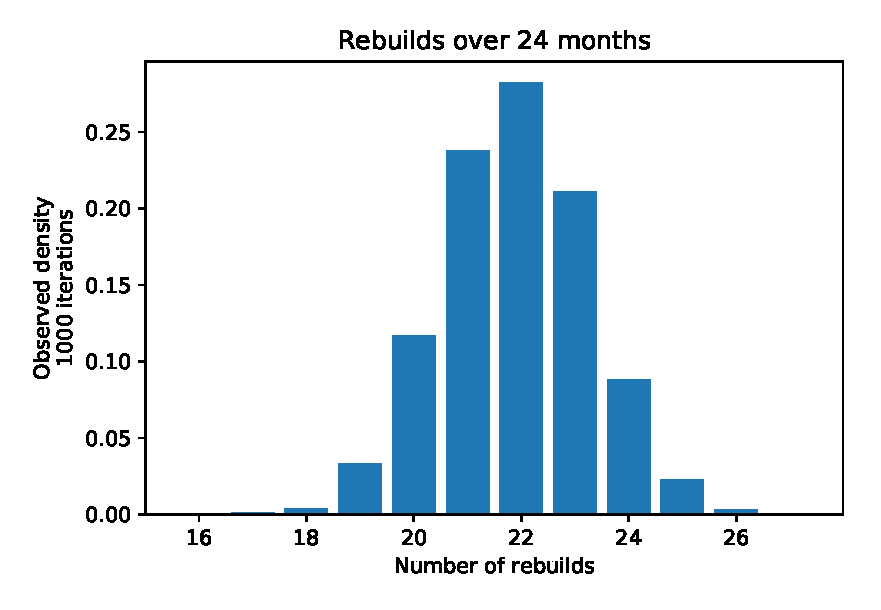
\includegraphics[scale=0.5]{RS-appendix-files/example_pmf.eps}
    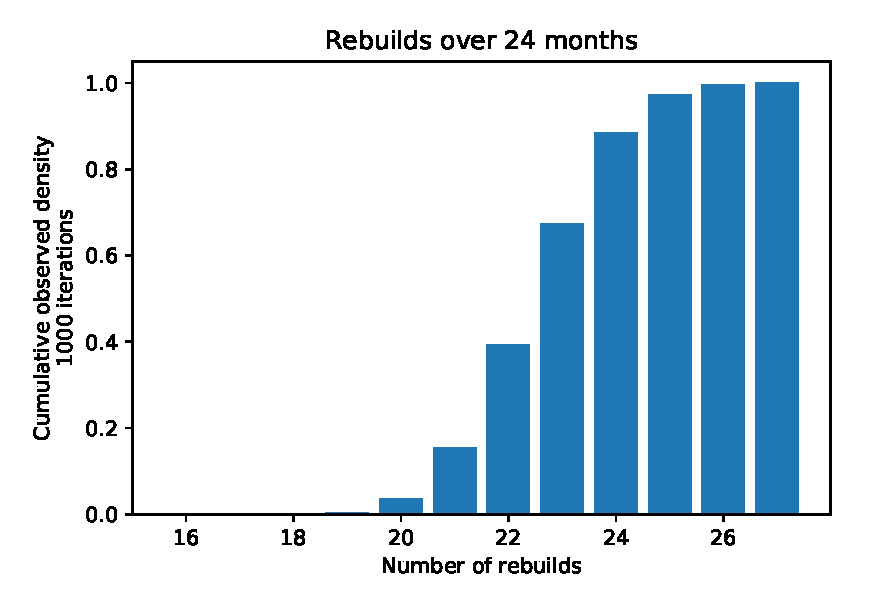
\includegraphics[scale=0.5]{RS-appendix-files/example_cdf.eps}
    \caption{Top: Density for the number of rebuilds over a 24 month period, repeated for 1000 iterations. Bottom: CDF of the number of rebuilds. In this case, the mean rebuilds/month value would be taken as $26/24\approx1.083$, with there being a 99.7\% chance that a file is rebuilt at most 26 times over the course of 24 months.}
    \label{fig:sim_method}
\end{figure}

\pagebreak
\linespread{1}
\pagebreak
\subsubsection{The decision tables}
In forming the decision tables, we consider as part of our calculations how
different choices of k, n, m, and mean time to failure affect durability and repair bandwidth. What we are looking for is the lowest repair bandwidth that also meets our
durability requirements.
\begin{table}[!htpb]\centering

\begin{tabular}{| c | c c c | c | c|}\hline
MTTF (months) &$k$& $n$ & $m$ &Repair Bandwidth Ratio&Durability (\# nines) \\\hline
1 &20& 40 & 35 & 9.36 & 0.9999 (8) \\
6 &20& 40 & 30 & 0.87 & 0.9999 (17) \\
12 &20& 40 & 25 & 0.31 & 0.9999 (13)\\\hline

1 &30& 60 & 35 & 3.40 &0.9999 (4)\\
6 &30& 70 & 40 & 0.60 &0.9999 (15)\\
12 &30& 80 & 45 & 0.31 &0.9999 (25) \\\hline

1 &40& 80 & 60 & 5.21 &0.9999 (4)\\
6 &40&120&50 & 0.52 &0.9999(14)\\
12 &40&120&45 & 0.24 &0.9999 (11)\\\hline

\end{tabular}
\caption{Decision tables showing the relationship between churn (MTTF),
  Reed-Solomon parameters ($k$, $n$, $m$), repair bandwidth ratio, and durability}
\label{rs:decision-tables}
\end{table}




\subsection{Making a decision}

We conclude by observing that these models may be tuned to target specific network scenarios and requirements. One network may require one set of Reed-Solomon parameters, while a different network may require another. In general, the closer $m/n$ is to 1, the more rebuilds per month should be expected under a fixed churn rate. While having a larger ratio for $m/n$ increases file durability for any given churn rate, it comes at the expense of more bandwidth used since repairs are triggered more often. To maintain a low mean rebuilds/month value while also maintaining a higher file durability, the aim should be to increase the value of $n$ as much as feasible given other network conditions (latency, download speed, etc.), which allows for a lower relative value of $r$ while still not jeopardizing file durability. 

Informally, it takes longer to lose more pieces under a given fixed network size and churn rate. Therefore, to maximize durability while minimizing repair bandwidth usage, $n$ should be as large as existing network conditions allow. This allows for a value of $m$ that is relatively closer to $k$, reducing the mean rebuilds/month value, which in turn lowers the amount of repair bandwidth used. 

For example, assume we have a network with a mean time to failure of six months.
Suppose we consider the same file encoded with two different RS parameters: 
one under a $(20,40)$ schema and the other as an $(30,80)$ schema. If we set $m$ so that $m=k+10$ for both cases, we observe from the above table
that the bandwidth repair ratio is is $0.87$ in the $(20,40)$ case and is $0.60$ in the $(40,80)$ case. Both encoding schemes have similar durability, as a repair in both cases is triggered when there are $k+10$ pieces left; even though, the mean rebuilds per month 
is empirically and theoretically lower for the $(40,80)$ case using $m=k+10$. 

\chapter{Distributed consensus}

\section{Non-byzantine}

A long and challenging area of research has been directed toward getting a
group of computers to agree on a set of values
\bs{what kind of values? principles? or numerical-type values?},
with the goal of constructing a
horizontally-scalable database that works in the face of expected failures
(crash failures, for example: failures where a server simply shuts down).
Fortunately, this research has led to some really exciting technology.

The biggest issue with getting a group of computers to agree is that messages
can be lost. How this impacts decision making is succinctly described by the
``Two Generals' Problem" \cite{two-generals}
\footnote{earlier described as a problem
between groups of gangsters \cite{two-gangsters}}, in which two armies try to
communicate in the face of potentially lost messages. Both armies have already
agreed to attack a shared enemy, but have yet to decide on a time. Both armies
must attack at the same time or else failure is assured. Both armies can send
messengers, but the messengers are often captured by the enemy. Both armies must
know what time to attack and that the other army has also agreed to this time.

Ultimately, a solution to the two generals' problem with a finite number of
messages is readily seen to be impossible, so engineering approaches have had
to embrace uncertainty by necessity. Many distributed systems make trade-offs to
deal with this uncertainty. Some systems embrace {\em consistency}, which means
that the system will choose downtime over inconsistent answers. Other
systems embrace {\em availability}, which means that the system chooses
potentially inconsistent answers over downtime. The widely-cited CAP
theorem \cite{cap1, cap2} states that every system must choose only two of
consistency, availability, and partition tolerance.
Due to the inevitability of network
failures, partition tolerance is non-negotiable, so when a partition happens,
every system must choose to sacrifice either consistency or availability. Many
systems sacrifice both (sometimes by accident).

In the CAP theorem, consistency means that every read receives the most recent
write or an error, so an inconsistent answer means the system returned something
besides the most recent write without obviously failing. More generally, there
are a number of {\em consistency models} that may be acceptable by making
various tradeoffs. Linearizability, sequential consistency, causal consistency,
PRAM consistency, eventual consistency, read-after-write consistency, etc., are
all models for discussing how a history of events appears to various
participants in a distributed system.\footnote{If differing consistency models
are new to you, it may be worth reading about them in Kyle Kingbury's excellent
tutorial \cite{aphyr-consistency}. If you're wondering why computers can't just
use the current time to order events, keep in mind it is exceedingly difficult
to get computers to even agree on that \cite{no-now}.}

Amazon S3 generally provides {\em read-after-write consistency}, though in some
cases will provide {\em eventual consistency} instead \cite{s3-consistency}.
Arguably, there may be some flexibility here which allows for the selection
of alternate consistency models that suit us better while still broadly
providing S3 compatibility.
Many distributed databases provide eventual consistency by
default, such as Dynamo \cite{dynamo} and Cassandra \cite{cassandra}.

Linearizability in a distributed system is often much more desirable
\bs{than what?}, as it is
useful as a building block for many higher level data structures and operations
such as distributed locks and other coordination techniques. Initially, early
efforts centered around two-phase commit, then three-phase commit, which both
suffered due to issues similar to the two generals' problem. Things were looking
bad in 1985 when the FLP-impossibility paper \cite{flp} proved that no algorithm
could reach linearizable consensus in bounded time. Then in 1988, Barbara Liskov
and Brian Oki published the Viewstamped Replication algorithm \cite{vr} which
was the first linearizable distributed consensus algorithm. Unaware of the VR
publication, Leslie Lamport set out to prove linearizable distributed consensus
was impossible \cite{paxos-note}, but instead in 1989 proved it was possible by
publishing his own Paxos algorithm \cite{paxos}, which for some reason became
significantly more popular. Ultimately both algorithms have a large amount in
common.

Despite Lamport's claims that Paxos is actually simple \cite{paxos-simple},
many papers have been published since then
challenging that assertion. Google's description of their attempts to implement
Paxos are described in Paxos Made Live \cite{paxos-live},
and Paxos Made Moderately
Complex \cite{paxos-complex} is an attempt to try and fill in all the details of
the protocol. The entire basis of the Raft algorithm is rooted in trying to
wrangle and simplify the complexity of Paxos \cite{raft}. Ultimately, after an
upsetting few decades, reliable implementations of Paxos, Raft, Viewstamped
Replication \cite{vrr}, Chain Replication \cite{chain-rep}, and Zab \cite{zab}
now exist, with ongoing work to improve the situation
further \cite{epaxos,paxos-flexible}. Arguably, part of Google's early success
was in spending the time to build their internal Paxos-as-a-service distributed
lock system, Chubby \cite{chubby}. Most of Google's most famous internal data
storage tools such as Bigtable \cite{bigtable} depend on Chubby for
correctness. Spanner \cite{spanner} -- perhaps one of the most incredible
distributed databases in the world -- is mainly just two-phase commit on top of
multiple Paxos groups.

Reliable distributed consensus algorithms have been game-changing for many
applications requiring fault-tolerant storage.

\section{Byzantine}

As mentioned in our design constraints, we expect most nodes to be {\em
rational} and some to be {\em byzantine}, but few-to-none to be {\em
altruistic}. Unfortunately, all of the previous algorithms we discussed assume a
collection of altruistic nodes.

There have been a number of attempts to solve the Byzantine fault tolerant
distributed consensus problem
(PBFT \cite{pbft} (Barbara Liskov again with the
first solution out of the gate), Q/U \cite{qu}, FaB \cite{fab} (but see
\cite{fab-revisited}), Bitcoin \cite{bitcoin}, Zyzzyva \cite{zyzzyva} (but also
see \cite{fab-revisited}), RBFT \cite{rbft}, Tangaroa \cite{tangaroa},
Tendermint \cite{tendermint}, Aliph \cite{aliph}, Hashgraph \cite{hashgraph},
HoneybadgerBFT\cite{honeybadger}, Algorand\cite{algorand}, Casper\cite{casper},
Tangle\cite{tangle}, Avalanche\cite{avalanche}, PARSEC\cite{parsec}, and
others\cite{mickens-bft}).
Each of these algorithms make some
additional tradeoffs that non-Byzantine distributed consensus algorithms don't
require to deal with the potential for uncooperative nodes. For example,
PBFT \cite{pbft} causes a significant amount of network overhead. Bitcoin
\cite{bitcoin} intentionally limits the transaction rate with changing
proof-of-work difficulty, in addition to requiring all participants to keep a
full copy of all change histories (like other blockchain-based
solutions).

\todo{talk about merkle-dag, git-inspired approaches to metadata, and how
they struggle with conflict resolution due to the lack of crdt-like options for
file systems}

\chapter{Object repair costs}

A fundamental question for networks relying on erasure coding and repair is
how to choose the best set of system parameters to obtain a desired level of
reliability under a given constraint of bandwidth consumption.

\todo{fill this in}

\chapter{Bandwidth availability limits usable space}\label{appendix:bandwidth-space-limits}

\todo{explain how bandwidth availability limits usable space (due to repair costs)}

\chapter{Audit false positive risk}\label{appendix:audit-false-positive}

\todo{calculate the risk of a false positive with an audit}

\chapter{TODO}

\todo{
New todo items:
\begin{itemize}
\item Clean up intro
\item Section \ref{sec:req-bandwidth} needs an appendix that explains how
  bandwidth availability and repair traffic limit usable space.
\item Section \ref{sec:framework-audits} needs an appendix on audit false
  positive calculations.
\end{itemize}

Old todo items:
\begin{itemize}
\item Datascience: write an appendix about repair bandwidth based on node
  churn and uptime
\item Datascience: Write an appendix about how we select RS numbers
\item Eng/marketing: Quality control/branding section - talk about how we
  plan to ensure satellite quality by quality control evaluations, formal
  partnerships, relationships, and not letting poor quality satellites
  use the brand.
\item tie framework back to design constraints
\item tie concrete implementation back to framework
\item Anyone:
  Clean up distributed consensus positioning in the appendix.
\item Eng: General data repair framework description
\item Eng: more macaroon details
\item Eng: future work section about hot files
\item make point about why rs is better than replication more clear,
  contrasting with other approaches
\item discuss when a storage node can limit download bandwidth to prevent
  abuse
\item Eng: Write a future work section about eliminating TLS handshakes
\item Eng: Write about how piece ids are generated
\item Eng: Future work section about reputation sharing
\item Eng: Future work section about finding a better data structure than
 a bloom filter for gc
\item Figure out latex theme licensing
\item Make sure audits try to refresh the cache if there's a failure contacting
  a node before flagging the node as down.
\end{itemize}
}

\newpage
\bibliographystyle{unsrt}
\begingroup
\raggedright
\bibliography{biblio}
\endgroup

\end{document}
